% ============================================================================
% TUGAS AKHIR - JALUR REGULER
% Template LaTeX laporan Tugas Akhir jalur Reguler
% Program Studi D3 Rekayasa Perangkat Lunak Aplikasi
% Fakultas Ilmu Terapan, Universitas Telkom
%
% Sumber: Template TA Reguler_4.docx (milik Prodi D3RPLA, tidak ikut dipush ke repo).
% Catatan: Jalur ini memiliki 2 Dosen Pembimbing (Pembimbing 1 + Reviewer).
% ============================================================================

\documentclass[a4paper,12pt,oneside]{report}

% --- Paket standar ---
\usepackage[a4paper,margin=3cm]{geometry}
\usepackage[onehalfspacing]{setspace}
\usepackage{array}
\usepackage{booktabs}
\usepackage{tabularx}
\usepackage{longtable}
\usepackage{multirow}
\usepackage{multicol}
\usepackage{graphicx}
\usepackage{float}
\usepackage{caption}
\usepackage{titlesec}
\usepackage{fancyhdr}
\usepackage{enumitem}
\usepackage{hyperref}
\usepackage{url}
\usepackage{listings}
\usepackage{xcolor}
\usepackage{amssymb} % menyediakan \checkmark

\hypersetup{colorlinks=true,linkcolor=black,urlcolor=blue,citecolor=black}
\captionsetup{font=small,labelfont=bf,labelsep=period}
\graphicspath{{assets/reguler/}{assets/}}

\titleformat{\chapter}[display]{\normalfont\huge\bfseries\filcenter}{BAB \thechapter}{0pt}{}
\titleformat{\section}{\normalfont\large\bfseries}{\thesection}{1em}{}
\titleformat{\subsection}{\normalfont\normalsize\bfseries}{\thesubsection}{1em}{}
\titleformat{\subsubsection}{\normalfont\normalsize\bfseries}{\thesubsubsection}{1em}{}

\usepackage{chngcntr}
\counterwithin{figure}{chapter}
\counterwithin{table}{chapter}
\renewcommand{\thefigure}{\arabic{chapter}.\arabic{figure}}
\renewcommand{\thetable}{\arabic{chapter}.\arabic{table}}

\pagestyle{fancy}
\fancyhf{}
\fancyhead[L]{\small\leftmark}
\fancyhead[R]{\raisebox{-0.1cm}{
\includegraphics[height=0.7cm]{header-logo}}}
\fancyfoot[C]{\thepage}
\renewcommand{\headrulewidth}{0.4pt}
\setlength{\headheight}{22pt}

% --- Style listing untuk source code ---
\lstset{
    basicstyle=\ttfamily\small,
    breaklines=true,
    frame=single,
    captionpos=b,
    tabsize=2,
    showstringspaces=false
}

\begin{document}

% =====================================================================
% HALAMAN COVER
% =====================================================================
\begin{titlepage}
    \centering
    \vspace*{1cm}
    {\bfseries\Large JUDUL TUGAS AKHIR DALAM BAHASA INDONESIA\\(maksimal 3 baris)\par}
    \vspace{1cm}
    {\bfseries\Large JUDUL TUGAS AKHIR DALAM BAHASA INGGRIS\\(maximum 3 lines)\par}
    \vspace{2cm}

    Dokumen ini ditujukan untuk memenuhi persyaratan\\
    Mata Kuliah Tugas Akhir\\
    \textbf{Jalur Reguler}\par
    \vspace{1cm}
    
\includegraphics[height=3cm]{cover-banner}\par
    \vspace{1cm}

    Disusun oleh,\\
    NIM - NAMA\par
    \vfill

    \textbf{PROGRAM STUDI}\\
    \textbf{D3 REKAYASA PERANGKAT LUNAK APLIKASI}\\
    \textbf{FAKULTAS ILMU TERAPAN}\\
    \textbf{UNIVERSITAS TELKOM}\\
    \textbf{BANDUNG}\\
    202\ldots\par
\end{titlepage}

% =====================================================================
% LEMBAR PERSEMBAHAN
% =====================================================================
\chapter*{Lembar Persembahan}
\addcontentsline{toc}{chapter}{LEMBAR PERSEMBAHAN}

\begin{center}
    Untuk orang tuaku,\\
    orang paling berjasa di seluruh dunia.
\end{center}

\vspace{3cm}
\begin{flushleft}
    Nama \#1\\
    Nama \#2
\end{flushleft}

% =====================================================================
% LEMBAR PENGESAHAN
% =====================================================================
\chapter*{Lembar Pengesahan}
\addcontentsline{toc}{chapter}{LEMBAR PENGESAHAN}

\noindent\textit{Pastikan kalimat dan penggalan judul sama persis dengan cover}

\begin{center}
    {\bfseries JUDUL TUGAS AKHIR DALAM BAHASA INDONESIA}\\[6pt]
    {\bfseries JUDUL TUGAS AKHIR DALAM BAHASA INGGRIS}
\end{center}

\vspace{1cm}
\begin{table}[h]
    \centering
    \begin{tabular}{p{4cm}p{8cm}}
        Penulis                 & Nama Lengkap Mahasiswa \\
        NIM                     & 60706.\ldots \\
        \multicolumn{2}{c}{} \\
        Dosen Pembimbing 1      & Nama Dosen Pembimbing \\
        NIP                     & 078\ldots\ldots \\
        \multicolumn{2}{c}{} \\
        Dosen Pembimbing 2      & Nama Dosen Reviewer \\
        NIP                     & 098\ldots\ldots \\
    \end{tabular}
\end{table}

\vspace{2cm}
\begin{center}
    Tanggal Pengesahan: 31 Juli 2025 (tanggal pengumpulan revisi)
\end{center}

% =====================================================================
% KATA PENGANTAR
% =====================================================================
\chapter*{Kata Pengantar}
\addcontentsline{toc}{chapter}{KATA PENGANTAR}

Berisi kata pengantar; dan ditulis dalam bahasa Indonesia baku.

\vspace{3cm}
\begin{flushright}
    Bandung, \textless\textless Bulan\textgreater\ \textless\textless Tahun\textgreater\textgreater\\[6pt]
    Penulis
\end{flushright}

% =====================================================================
% PERNYATAAN
% =====================================================================
\chapter*{Pernyataan}
\addcontentsline{toc}{chapter}{PERNYATAAN}

Dengan ini saya menyatakan bahwa:
\begin{enumerate}[label=\arabic*.]
    \item Karya tulis ini adalah asli dan belum pernah diajukan untuk mendapatkan
    gelar akademik (Ahli Madya, Sarjana, Magister dan Doktor), baik di Fakultas
    Ilmu Terapan Universitas Telkom maupun di perguruan tinggi lainnya;
    \item karya tulis ini murni gagasan, rumusan, dan penelitian saya sendiri,
    tanpa bantuan pihak lain, kecuali arahan tim pembimbing atau tim promotor
    atau penguji;
    \item dalam karya tulis ini tidak terdapat cuplikan karya atau pendapat yang
    telah ditulis atau dipublikasikan orang lain, kecuali secara tertulis dengan
    jelas dicantumkan sebagai acuan dalam naskah dengan menyebutkan nama
    pengarang dan dicantumkan dalam daftar pustaka;
    \item saya mengijinkan karya tulis ini dipublikasikan oleh Fakultas Ilmu
    Terapan Universitas Telkom, dengan tetap mencantumkan saya sebagai penulis;
    dan
    \item Pernyataan ini saya buat dengan sesungguhnya dan apabila pada kemudian
    hari terdapat penyimpangan dan ketidakbenaran dalam pernyataan ini maka saya
    bersedia menerima sanksi akademik berupa pencabutan gelar yang telah
    diperoleh karena karya tulis ini, serta sanksi lainnya sesuai norma yang
    berlaku di Fakultas Ilmu Terapan Universitas Telkom.
\end{enumerate}

\vspace{2cm}
\begin{flushright}
    Bandung, 31 Juli 2025 (tanggal pengumpulan revisi)\\[6pt]
    Pembuat pernyataan,\\[3cm]
    (tulis nama jelas di sini tanpa gelar)
\end{flushright}

% =====================================================================
% ABSTRAK
% =====================================================================
\chapter*{Abstrak}
\addcontentsline{toc}{chapter}{ABSTRAK}

Abstrak adalah representasi dari isi dokumen yang singkat dan tepat. Tujuan
abstrak adalah memudahkan pembaca mendapatkan informasi mengenai Tugas Akhir
yang dibuat penulis tanpa harus membaca seluruh isi dokumen serta menghemat
waktu pembaca. Abstrak ditulis dalam 1 paragraf saja, dengan panjang tidak
lebih dari 250 (dua ratus lima puluh) kata dengan spacing 1. Abstrak tidak
mencantumkan landasan teori. Abstrak harus dibuat dengan ringkas dan mampu
menggambarkan alasan atau pentingnya Tugas Akhir ini, tujuan yang hendak
dicapai (atau fitur-fitur utama yang ada dalam produk Tugas Akhir),
langkah-langkah metode pengerjaannya, tools yang digunakan, dan kesimpulan.

\vspace{1cm}
\noindent\textbf{Kata Kunci:} (keywords abstrak 5-6 kata/frasa)

% =====================================================================
% ABSTRACT
% =====================================================================
\chapter*{Abstract}
\addcontentsline{toc}{chapter}{ABSTRACT}

\begin{spacing}{1}
\textit{Write your abstract in English. Using spacing 1 and italic.\\
DO NOT USE ENGLISH TRANSLATOR SOFTWARE WITHOUT FURTHER EDITING}

\vspace{1cm}
\noindent\textbf{Keywords:} (abstract keywords 5-6 words/phrases)
\end{spacing}

% =====================================================================
% DAFTAR ISI / GAMBAR / TABEL / LAMPIRAN
% =====================================================================
\tableofcontents
\listoffigures
\listoftables

\chapter*{Daftar Lampiran}
\addcontentsline{toc}{chapter}{DAFTAR LAMPIRAN}
\begin{enumerate}[label=Lampiran \arabic*.,leftmargin=*]
    \item Dokumentasi Kegiatan
    \item Perhitungan Usability Test
\end{enumerate}

% =====================================================================
% BAB I PENDAHULUAN
% =====================================================================
\chapter{Pendahuluan}

\section{Latar Belakang}
Latar belakang diawali dengan menceritakan masalah yang menjadi alasan kenapa
tugas akhir ini dibuat. Menceritakan masalahnya harus didukung dengan
data/artikel yang sumbernya dapat dipertanggungjawabkan. Masukkan referensi yang
dipakai ke dalam daftar pustaka menggunakan format yang baku. Setelah
menceritakan masalah, lanjutkan dengan menceritakan secara singkat solusi atas
permasalahan tersebut. Latar belakang dibuat antara 1 -- 1,5 halaman saja, dibagi
ke dalam beberapa paragraf yang panjangnya kurang lebih sama. Contoh:

Berdasarkan data yang dihimpun oleh Kementerian Kesehatan, penyandang
disabilitas di Indonesia kurang lebih berjumlah 6 juta jiwa, dimana di dalamnya
terdapat sekitar 472 ribu jiwa penyandang tunarungu~\cite{ref1}. Tunarungu adalah
suatu kondisi dimana seseorang mengalami kekurangan indra pendengaran sehingga
tidak mampu menangkap bunyi. Sebagai akibat terhambatnya perkembangan pendengaran,
seorang tunarungu biasanya juga terhambat kemampuan bicara dan bahasanya,
sehingga seorang tunarungu akan mengalami kelambatan dan kesulitan dalam hal
komunikasi~\cite{ref2}.

Di Indonesia, bahasa isyarat yang digunakan oleh kalangan tunarungu untuk
komunikasi terdapat dua jenis yaitu Bahasa Isyarat Indonesia (BISINDO) dan
Sistem Isyarat Bahasa Indonesia (SIBI). SIBI merupakan bahasa yang biasa
dipakai di Sekolah Luar Biasa (SLB) karena SIBI merupakan bahasa isyarat yang
resmi berdasarkan aturan bahasa isyarat di Indonesia. Terdapat sebanyak 2.070
SLB di seluruh Indonesia dengan jumlah siswa penyandang tunarungu sebanyak
24.374 siswa, yang merupakan siswa penyandang disabilitas terbanyak kedua di
Indonesia setelah tunagrahita~\cite{ref3}.

Namun sayangnya, pembelajaran kosakata baru SIBI pada SLB masih menggunakan
cara konvensional yaitu masih menggunakan kamus bahasa isyarat, dimana kamus
tersebut harganya mencapai 2,5 juta rupiah~\cite{ref4} dan sulit dimengerti
karena hanya menggunakan gambar dengan panduan gerakan berupa teks keterangan.
Apalagi di masa pandemi, pembelajaran harus dilakukan secara daring, sehingga
mengganggu proses pembelajaran karena siswa sangat bergantung pada visual dalam
belajar. Apabila koneksi internet siswa sedang tidak stabil, maka itu akan
mengganggu proses pembelajaran.

Oleh karena itu dibuatlah aplikasi yang bernama SIBIKU, yaitu sebuah aplikasi
Android yang merupakan Kamus Sistem Isyarat Bahasa Indonesia (SIBI) dengan
gambar bergerak dan dilengkapi dengan morse getaran. Aplikasi ini dibuat dengan
tujuan agar dapat membantu anak-anak penyandang tunarungu untuk belajar
kosakata bahasa isyarat. Pada aplikasi SIBIKU terdapat beberapa fitur yang
berbeda dengan aplikasi-aplikasi yang sudah ada, namun utamanya yaitu fitur kata
menggunakan gambar bergerak yang bisa ditambah kapan saja oleh guru/admin dari
aplikasi SIBIKU Admin.

Fitur lainnya yaitu fitur huruf dan angka yang bisa dikonversi menjadi morse
yang berbentuk getaran dan fitur kuis tebak kata agar menambah semangat belajar
pengguna dan sebagai bahan evaluasi dalam pembelajaran kosakata yang sedang
dipelajari. Dengan adanya aplikasi SIBIKU ini diharapkan dapat membantu
menyelesaikan masalah yang dihadapi oleh guru dan siswa penyandang tunarungu
dalam pembelajaran kosakata isyarat sehingga tidak perlu lagi membeli kamus yang
tebal, mahal dan sulit untuk didapat dan juga membantu dalam pembelajaran
kosakata baru.

\section{Rumusan Masalah}
Uraikan pendekatan dan konsep untuk menjawab masalah yang diteliti, masalah
yang akan dicari penyelesaiannya. Contoh:

Berdasarkan latar belakang di atas, maka rumusan masalah yang akan dibahas:
\begin{itemize}
    \item Bagaimana siswa SLB dapat belajar kosakata bahasa isyarat dengan mudah?
    \item Bagaimana cara membantu sekolah dan guru dalam pembelajaran kosakata
    baru pada siswa penyandang tunarungu?
    \item Bagaimana merancang sebuah aplikasi yang memudahkan siswa SLB dalam
    belajar kosakata baru?
\end{itemize}

\section{Tujuan}
Berikan pernyataan singkat mengenai tujuan TA. Tujuan hendaknya jelas, dapat
diukur serta memiliki korelasi yang erat dengan rumusan masalah. Contoh:

Berdasarkan rumusan masalah yang ada, tujuan yang akan dicapai adalah:
\begin{itemize}
    \item Aplikasi dapat membantu penyandang tunarungu untuk lebih mudah belajar
    bahasa isyarat dengan Sistem Isyarat Bahasa Indonesia (SIBI).
    \item Membantu sekolah dan guru dalam pembelajaran kosakata baru pada siswa
    penyandang tunarungu.
    \item Merancang aplikasi kamus SIBI berbasis Android.
\end{itemize}

\section{Batasan Masalah}
Dalam perumusan masalah dapat dijelaskan definisi, asumsi, dan lingkup yang
menjadi batasan TA. Contoh:

Batasan masalah dalam pembuatan aplikasi ini adalah:
\begin{itemize}
    \item Aplikasi diimplementasikan pada smartphone Android minimal versi Lollipop.
    \item Kata isyarat yang digunakan dalam aplikasi adalah kata isyarat tingkat SD.
    \item Keberlanjutan kata isyarat yang diinput sesuai dengan kesepakatan guru/admin.
    \item Pengguna dikhususkan bagi penyandang tunarungu yang bersekolah di SD.
    \item Bahasa isyarat menggunakan Sistem Isyarat Bahasa Indonesia.
\end{itemize}

\section{Metode Penyelesaian Masalah}
Uraian metodologi penyelesaian masalah dapat berupa variabel-variabel dalam
penelitian, model yang digunakan, rancangan penelitian, teknik pengumpulan data
dan analisis data, cara penafsiran dan penyimpulan hasil penelitian. Tiap tahap
penyelesaian masalah harus sudah berisi dengan detil dan lengkap dari kegiatan
yang dilakukan dalam penyelesaian TA. Contoh:

Berikut metodologi penyelesaian masalah yang digunakan dalam tugas akhir ini.

\textbf{Studi Literatur}\\
Mencari referensi yang berhubungan dengan topik tugas akhir ini seperti kondisi
pengajaran di SLB, karakteristik pengguna tunarungu dan bahasa isyarat SIBI
dalam bentuk buku, jurnal, paper, dan sumber tertulis lainnya. Selain itu, juga
mempelajari dan memahami materi yang berhubungan dengan topik tugas akhir
seperti platform Android dan database yang akan dipakai.

\textbf{Analisis Kebutuhan}\\
Melakukan komunikasi dengan pihak SLB terkait dengan sistem pembelajaran
tunarungu di SLB sehingga akan didapatkan data yang sesuai dengan permasalahan
yang dialami pengguna, dalam hal ini guru dan siswa penyandang tunarungu. Selain
itu juga untuk membantu dalam menentukan fitur yang dibutuhkan oleh pengguna
pada aplikasi yang akan dikembangkan.

\textbf{Perancangan Aplikasi}\\
Melakukan perancangan aplikasi SIBIKU berdasarkan analisa kebutuhan dan studi
literatur yang telah dilakukan. Di tahap ini paling tidak akan ditentukan
fitur-fitur yang akan diimplementasikan dalam aplikasi, rancangan tampilan
aplikasi, dan struktur basis data yang akan dipakai di aplikasi.

\textbf{Pembuatan Aplikasi}\\
Pada tahap ini melakukan pembuatan aplikasi dengan cara koding sesuai dengan
perancangan aplikasi yang telah dibuat. Dalam proses pembuatan aplikasi, tools
yang digunakan meliputi Android Studio, Firebase, dan SQLite dengan menggunakan
bahasa Kotlin dan arsitektur MVVM.

\textbf{Pengujian Aplikasi}\\
Pada tahapan ini dilakukan pengujian untuk mengobservasi kesalahan yang mungkin
terjadi pada aplikasi, sehingga dapat dipastikan aplikasi berjalan sesuai dengan
yang diharapkan. Pengujian dilakukan dua tahap, pertama oleh developer aplikasi,
kemudian dengan mitra dan pengguna lainnya.

\section{Pembagian Tugas Akhir}
\textit{Subbab ini bersifat opsional dan hanya ada jika satu project dipecah
pengerjaannya menjadi lebih dari satu judul tugas akhir. Apabila 1 project
dikerjakan sendiri saja, maka subbab ini dapat dihapus.}

Berikut adalah pembagian pekerjaan tim tugas akhir:

\textbf{Judul Tugas Akhir 1}\\
Dikerjakan oleh: Nama mahasiswa 1\\
Penjelasan singkat mengenai TA 1\ldots

\textbf{Judul Tugas Akhir 2}\\
Dikerjakan oleh: Nama mahasiswa 2\\
Penjelasan singkat mengenai TA 2\ldots

% =====================================================================
% BAB II TINJAUAN PUSTAKA
% =====================================================================
\chapter{Tinjauan Pustaka}

\section{Teori A}
Tinjauan pustaka berisi teori-teori yang akan digunakan dalam pengerjaan tugas
akhir. Jadi bukan tentang sejarah sebuah framework atau tools tertentu. Sebagai
contoh, ketika membahas tentang Android, fokus bahasan bukan tentang Android
dibuat oleh siapa, diakuisisi sama siapa dan kapan kejadiannya. Tapi bahasalah
tentang komponen aplikasi Android seperti activity, services, broadcast receiver
dan content provider yang mungkin akan dipakai di aplikasi kalian nantinya.

Lorem ipsum dolor sit amet, consectetur adipiscing elit. Proin in porttitor
augue, vitae accumsan purus. Class aptent taciti sociosqu ad litora torquent per
conubia nostra, per inceptos himenaeos. Etiam pulvinar cursus magna vel eleifend.
Nunc gravida elit sed lectus accumsan tempus. Fusce et convallis magna, at
viverra ligula. Praesent rhoncus venenatis mattis. Sed maximus tortor tortor.

Curabitur id ullamcorper risus. Mauris in gravida libero, a lacinia ligula.
Donec consectetur purus non lectus eleifend, eu vehicula odio cursus.
Suspendisse potenti. Quisque quis erat in nunc fermentum fringilla quis eget
dui. Donec tortor odio, tincidunt ac faucibus eget, elementum eget massa. Sed ac
ante ac nulla maximus lobortis a vel dui. Pellentesque pellentesque in orci id
finibus.

\begin{figure}[H]
    \centering
    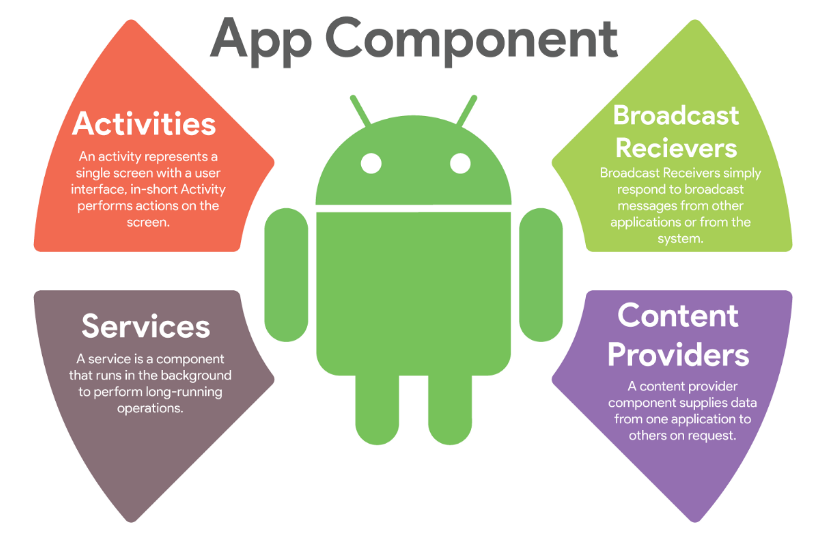
\includegraphics[width=0.85\textwidth]{komponen-android}
    \caption{Komponen Aplikasi Android}
    \label{fig:komponen-android}
\end{figure}

Setiap gambar harus dirujuk di dalam paragraf. Pakai menu References > Insert
Caption di Microsoft Word untuk memberi keterangan gambar agar daftar gambar
bisa dibuat secara otomatis. Gunakan format seperti di atas.

Semua sumber studi literatur harus ditulis lengkap dan jelas seperti yang
tercantum pada Daftar Pustaka. Penulisan literatur menggunakan style IEEE.
Berikut adalah contoh yang benar dalam mengutip definisi atau informasi dari
sebuah literatur.

\section{Teori B}
Lorem ipsum dolor sit amet, consectetur adipiscing elit. Proin in porttitor
augue, vitae accumsan purus. Class aptent taciti sociosqu ad litora torquent per
conubia nostra, per inceptos himenaeos. Etiam pulvinar cursus magna vel eleifend.
Nunc gravida elit sed lectus accumsan tempus. Fusce et convallis magna, at
viverra ligula. Praesent rhoncus venenatis mattis. Sed maximus tortor tortor.
Curabitur id ullamcorper risus. Mauris in gravida libero, a lacinia ligula.

Donec consectetur purus non lectus eleifend, eu vehicula odio cursus.
Suspendisse potenti. Quisque quis erat in nunc fermentum fringilla quis eget
dui. Donec tortor odio, tincidunt ac faucibus eget, elementum eget massa. Sed ac
ante ac nulla maximus lobortis a vel dui. Pellentesque pellentesque in orci id
finibus. Pellentesque efficitur arcu nec dolor feugiat bibendum in ut quam.
Aliquam pharetra urna neque, quis auctor lacus pellentesque a. Duis viverra eros
mi.

\section{Teori C}
Lorem ipsum dolor sit amet, consectetur adipiscing elit. Proin in porttitor
augue, vitae accumsan purus. Class aptent taciti sociosqu ad litora torquent per
conubia nostra, per inceptos himenaeos. Etiam pulvinar cursus magna vel eleifend.
Nunc gravida elit sed lectus accumsan tempus. Fusce et convallis magna, at
viverra ligula. Praesent rhoncus venenatis mattis. Sed maximus tortor tortor.

Curabitur id ullamcorper risus. Mauris in gravida libero, a lacinia ligula.
Donec consectetur purus non lectus eleifend, eu vehicula odio cursus.
Suspendisse potenti. Quisque quis erat in nunc fermentum fringilla quis eget
dui. Donec tortor odio, tincidunt ac faucibus eget, elementum eget massa. Sed ac
ante ac nulla maximus lobortis a vel dui. Pellentesque pellentesque in orci id
finibus.

\section{Aplikasi Serupa}
Bagian ini berisi review dari aplikasi yang serupa dengan aplikasi tugas akhir
kalian. Install dan pakailah aplikasi serupa tersebut di perangkat kalian, coba
semua fiturnya, lalu tuliskan review aplikasi tersebut di sini. Ketika mencoba
aplikasi, jangan lupa lakukan screen recording untuk dokumentasi ya, karena akan
ditanyakan pada saat monev kedua.

Aplikasi yang serupa dengan tugas akhir ini yaitu:

\subsection{Aplikasi A}
\textbf{Deskripsi aplikasi:} Lorem ipsum dolor sit amet, consectetur adipiscing
elit. Proin in porttitor augue, vitae accumsan purus. Class aptent taciti
sociosqu ad litora torquent per conubia nostra, per inceptos himenaeos. Etiam
pulvinar cursus magna vel eleifend. Nunc gravida elit sed lectus accumsan tempus.
Fusce et convallis magna, at viverra ligula. Praesent rhoncus venenatis mattis.

\textbf{Link aplikasi:}\\
\url{https://play.google.com/store/apps/details?id=com.indraazimi.pengeluaran}

\textbf{Kelebihan aplikasi:} Lorem ipsum dolor sit amet, consectetur adipiscing
elit. Proin in porttitor augue, vitae accumsan purus. Class aptent taciti
sociosqu ad litora torquent per conubia nostra, per inceptos himenaeos. Etiam
pulvinar cursus magna vel eleifend. Nunc gravida elit sed lectus accumsan tempus.

\textbf{Kekurangan aplikasi:} Lorem ipsum dolor sit amet, consectetur adipiscing
elit. Proin in porttitor augue, vitae accumsan purus. Class aptent taciti
sociosqu ad litora torquent per conubia nostra, per inceptos himenaeos. Etiam
pulvinar cursus magna vel eleifend. Nunc gravida elit sed lectus accumsan tempus.

\subsection{Aplikasi B}
\textbf{Deskripsi aplikasi:} \ldots\\
\textbf{Link aplikasi:} \ldots\\
\textbf{Kelebihan aplikasi:} \ldots\\
\textbf{Kekurangan aplikasi:} \ldots

\subsection{Aplikasi C}
\textbf{Deskripsi aplikasi:} \ldots\\
\textbf{Link aplikasi:} \ldots\\
\textbf{Kelebihan aplikasi:} \ldots\\
\textbf{Kekurangan aplikasi:} \ldots

\subsection{Perbandingan Fitur}
Setelah melakukan review, fitur-fitur dari aplikasi di atas dapat disajikan
dalam Tabel~\ref{tab:perbandingan-fitur}. Tabel ini juga memuat rencana fitur
yang akan dikembangkan di tugas akhir ini.

\begin{table}[H]
    \caption{Perbandingan Fitur Aplikasi Serupa}
    \label{tab:perbandingan-fitur}
    \centering
    \footnotesize
    \begin{tabular}{|c|p{3.2cm}|c|c|c|c|}
        \hline
        \textbf{No.} & \textbf{Fitur Aplikasi} & \textbf{Aplikasi A} & \textbf{Aplikasi B} & \textbf{Aplikasi C} & \textbf{Aplikasi TA ini} \\ \hline
        1  & Fitur 1   & \checkmark & \checkmark &            & \checkmark \\ \hline
        2  & Fitur 2   & \checkmark &            & \checkmark & \checkmark \\ \hline
        3  & Fitur 3   &            &            & \checkmark & \checkmark \\ \hline
        \ldots & Fitur \ldots &        & \checkmark &            & \checkmark \\ \hline
        \ldots & Fitur \ldots & \checkmark & \checkmark & \checkmark & \checkmark \\ \hline
        dst & dst       &            &            & \checkmark &            \\ \hline
    \end{tabular}
\end{table}

\noindent\textit{Catatan: Rencana fitur aplikasi TA pada tabel di atas masih
boleh berubah. Jadi tidak perlu khawatir seandainya setelah dilakukan analisis
kebutuhan pengguna di Bab III, ternyata kebutuhan pengguna berbeda dari yang
dibayangkan.}

% =====================================================================
% BAB III ANALISIS KEBUTUHAN DAN PERANCANGAN
% =====================================================================
\chapter{Analisis Kebutuhan dan Perancangan}

\section{Analisis Kebutuhan Pengguna}
Analisis ini diawali dengan menggali kebutuhan pengguna, memahami karakteristik
mereka, dan menerjemahkan kebutuhan tadi menjadi fitur aplikasi.

\subsection{Proses Menggali Informasi}
Bagian ini setidaknya harus menjelaskan 4 hal yaitu: (a) apa metode yang
digunakan untuk menggali kebutuhan pengguna; (b) kapan dan dimana kegiatan
dilakukan; (c) siapa yang menjadi narasumber; serta (d) daftar pertanyaan yang
diajukan dan dasarnya. Lampirkan bukti kegiatan di Lampiran A. Contoh:

Informasi kebutuhan pengguna dan karakteristiknya digali dengan metode
wawancara. Wawancara dilaksanakan pada 30 November 2020 bertempat di SLB Negeri
Cicendo, Bandung. Wawancara dilakukan terhadap 1 orang siswa, 1 orang tua
siswa, dan 2 orang guru. Siswa yang diwawancarai merupakan siswa yang dipilih
oleh guru. Dokumentasi wawancara berupa foto kegiatan dapat dilihat di Lampiran A.

Pertanyaan yang diajukan dalam wawancara disusun berdasarkan teori-teori yang
telah ditinjau di Bab 2, aplikasi serupa yang telah di-review kelebihan dan
kekurangannya, serta sumber lain yang relevan. Daftar pertanyaan yang diajukan
dapat dilihat pada Tabel~\ref{tab:daftar-pertanyaan}.

\begin{table}[H]
    \caption{Daftar Pertanyaan yang Diajukan}
    \label{tab:daftar-pertanyaan}
    \centering
    \footnotesize
    \begin{tabular}{|c|p{6cm}|p{3cm}|}
        \hline
        \textbf{No.} & \textbf{Pertanyaan yang Diajukan} & \textbf{Narasumber} \\ \hline
        1 & Pertanyaan 1 & Siswa \\ \hline
        2 & Pertanyaan 2 & Siswa \\ \hline
        3 & Pertanyaan 3 & Siswa \\ \hline
        4 & Pertanyaan 4 & Ortu  \\ \hline
        5 & Pertanyaan 5 & Ortu  \\ \hline
        6 & Pertanyaan 6 & Ortu  \\ \hline
        7 & Pertanyaan 7 & Guru  \\ \hline
        8 & Pertanyaan 8 & Guru  \\ \hline
        9 & Pertanyaan 9 & Guru  \\ \hline
        \ldots & \ldots & \ldots \\ \hline
        dst & dst & dst \\ \hline
    \end{tabular}
\end{table}

\subsection{Karakteristik Target Pengguna}
Bagian ini setidaknya harus menjelaskan 3 hal yaitu: (a) siapa target pengguna
aplikasi; (b) bagaimana literasi mereka terhadap teknologi; dan (c) perangkat
yang dimiliki untuk mengakses aplikasi yang akan dikembangkan. Contoh:

Aplikasi ini dibuat untuk penyandang tunarungu, khususnya untuk anak-anak SLB
yang masih duduk di bangku sekolah dasar. Berdasarkan wawancara yang dilakukan,
diketahui bahwa anak-anak ini telah terbiasa menggunakan aplikasi yang ada pada
smartphone, terutama sejak adanya pandemi Covid-19 dimana sekolah diadakan
secara daring. Hanya saja, ketika di awal, umumnya orang tua harus mendampingi
terlebih dahulu sampai anak-anak itu terbiasa dan dapat menggunakan aplikasi
secara mandiri.

Smartphone yang digunakan biasanya adalah smartphone milik orang tua mereka
yang memiliki akses internet, walaupun terbatas karena sebagian besar hanya
menggunakan paket data. Spesifikasi target perangkat di
Tabel~\ref{tab:spesifikasi-perangkat} telah dikonfirmasi tersedia dan dapat
digunakan oleh anak-anak untuk memakai aplikasi yang akan dibangun.

\begin{table}[H]
    \caption{Spesifikasi Target Perangkat}
    \label{tab:spesifikasi-perangkat}
    \centering
    \begin{tabular}{|p{3.5cm}|p{8cm}|}
        \hline
        \textbf{Jenis} & \textbf{Spesifikasi Minimal} \\ \hline
        Perangkat keras & Smartphone dengan layar 4,7'', RAM 2GB dan internal memory 16GB \\ \hline
        Perangkat lunak & Sistem operasi Android minimal versi 5.0 (Lollipop, API level 21) \\ \hline
    \end{tabular}
\end{table}

\subsection{Fitur yang Dibutuhkan}
Bagian ini berisi mengenai analisis mengapa sebuah fitur di aplikasi perlu
dibangun? Apa kebutuhan pengguna yang mendasarinya? Kemudian bagaimana harapan
dari pengguna terhadap fitur tersebut? Jelaskan dalam poin-poin. Contoh:

Berdasarkan informasi kebutuhan yang telah digali, fitur aplikasi yang perlu
dibangun sesuai kebutuhan pengguna dapat diuraikan sebagai berikut.

\textbf{Fitur kata isyarat}
\begin{itemize}
    \item Media pembelajaran konvensional saat ini berupa gambar statis. Untuk
    memberi nilai tambah, aplikasi akan memuat gambar bergerak sehingga dapat
    memudahkan pengguna menirukan kata isyarat yang sedang dipelajari.
    \item Oleh karena aset gambar bergerak belum ada, disepakati yang akan
    menjadi model adalah siswa berprestasi yang dipilih oleh guru. Ini juga
    bertujuan agar pengguna lebih semangat belajar karena modelnya juga anak-anak.
    \item Aset gambar bergerak harus berukuran kecil agar tidak memberatkan
    smartphone. Ini disiasati dengan menggunakan aset dalam format GIF karena
    memiliki tingkat kompresi yang baik dan juga aset tidak memerlukan audio.
    \item Kata isyarat akan dikelompokkan ke dalam kategori tertentu sehingga
    guru akan lebih mudah mengarahkan siswanya ketika belajar.
\end{itemize}

\textbf{Fitur bla..bla..bla..}\\
Lorem ipsum dolor sit amet, consectetur adipiscing elit. Proin in porttitor
augue, vitae accumsan purus. Class aptent taciti sociosqu ad litora torquent per
conubia nostra, per inceptos himenaeos. Etiam pulvinar cursus magna vel
eleifend. Nunc gravida elit sed lectus accumsan tempus. Fusce et convallis magna.
At viverra ligula. Praesent rhoncus venenatis mattis. Sed maximus tortor tortor.
Curabitur id ullamcorper risus. Mauris in gravida libero, a lacinia ligula.
Donec consectetur purus non lectus eleifend.

\textbf{Fitur bla..bla..bla..}\\
Lorem ipsum dolor sit amet, consectetur adipiscing elit. Proin in porttitor
augue, vitae accumsan purus. Class aptent taciti sociosqu ad litora torquent per
conubia nostra, per inceptos himenaeos. Etiam pulvinar cursus magna vel
eleifend. Nunc gravida elit sed lectus accumsan tempus. Fusce et convallis magna.
At viverra ligula. Praesent rhoncus venenatis mattis. Sed maximus tortor tortor.
Curabitur id ullamcorper risus. Mauris in gravida libero, a lacinia ligula.
Donec consectetur purus non lectus eleifend.

\section{Perancangan Aplikasi}
Setelah karakteristik target pengguna dipahami dan fitur-fitur yang dibutuhkan
pengguna berhasil dirumuskan, aplikasi dirancang sebagai berikut.

\subsection{Gambaran Umum Aplikasi}
Jelaskan arsitektur aplikasi secara umum! Berupa aplikasi stand-alone, aplikasi
client-server, atau seperti apa? Bagian ini wajib memuat minimal 1 buah gambar
arsitektur aplikasi, dan setiap komponennya harus diceritakan. Contoh:

Aplikasi Android yang dirancang diberi nama SIBIKU dan akan terdiri dari dua
bagian yaitu aplikasi untuk siswa dan aplikasi untuk guru (admin) seperti
terlihat pada Gambar~\ref{fig:arsitektur-aplikasi}. Aplikasi guru akan terhubung
ke layanan Firebase Realtime Database dimana data kata isyarat untuk seluruh
pengguna disimpan. Aplikasi guru juga akan terhubung ke layanan Firebase Cloud
Storage, tempat dimana aset berupa gambar bergerak disimpan. Aplikasi guru akan
memiliki akses baca dan tulis ke kedua layanan ini.

\begin{figure}[H]
    \centering
    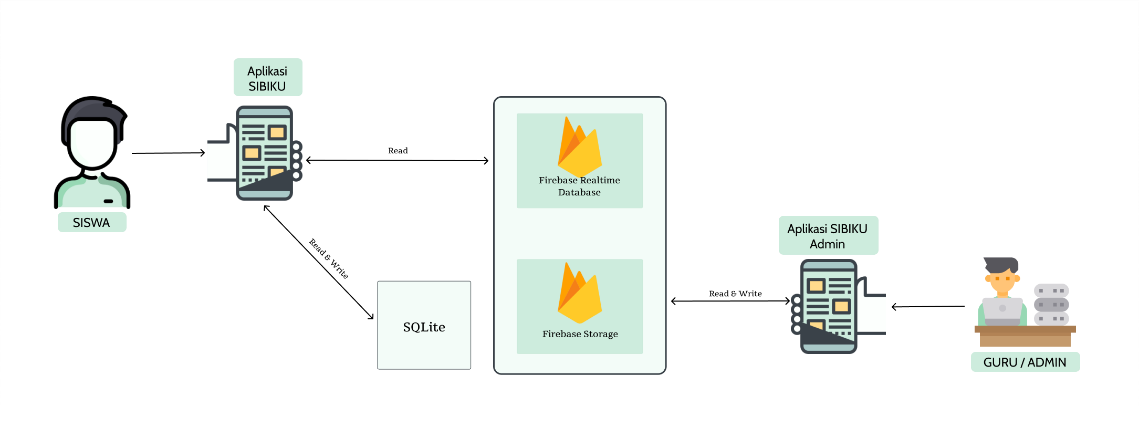
\includegraphics[width=0.85\textwidth]{arsitektur-aplikasi}
    \caption{Arsitektur Aplikasi}
    \label{fig:arsitektur-aplikasi}
\end{figure}

Di sisi lain, aplikasi untuk siswa akan memiliki hak akses baca saja ke layanan
Firebase Realtime Database dan Firebase Cloud Storage. Ketika siswa ingin
menambahkan kata isyarat baru, data kata tersebut akan disimpan di database
lokal SQLite. Sedangkan aset gambar bergeraknya akan disimpan di internal storage
smartphone. Dengan arsitektur ini, semua fitur yang dibutuhkan pengguna dapat
diakomodir.

\subsection{Use Case Diagram}
Diagram yang dibuat harus dapat menggambarkan semua fitur yang dibutuhkan oleh
pengguna sesuai hasil analisis di subbab 3.1.3. Diagram harus dijelaskan dalam
paragraf. Jadi bagian ini tidak boleh hanya berisi gambar. Contoh:

Berdasarkan kebutuhan pengguna yang telah dianalisis, fitur-fitur dalam aplikasi
dapat disajikan dalam use case diagram seperti tampak pada
Gambar~\ref{fig:usecase}. Terdapat dua orang aktor, yaitu siswa sebagai client
dan guru sebagai admin. Admin hanya dapat mengelola kata isyarat, dan client
dapat melakukan bla..bla..bla\ldots

\begin{figure}[H]
    \centering
    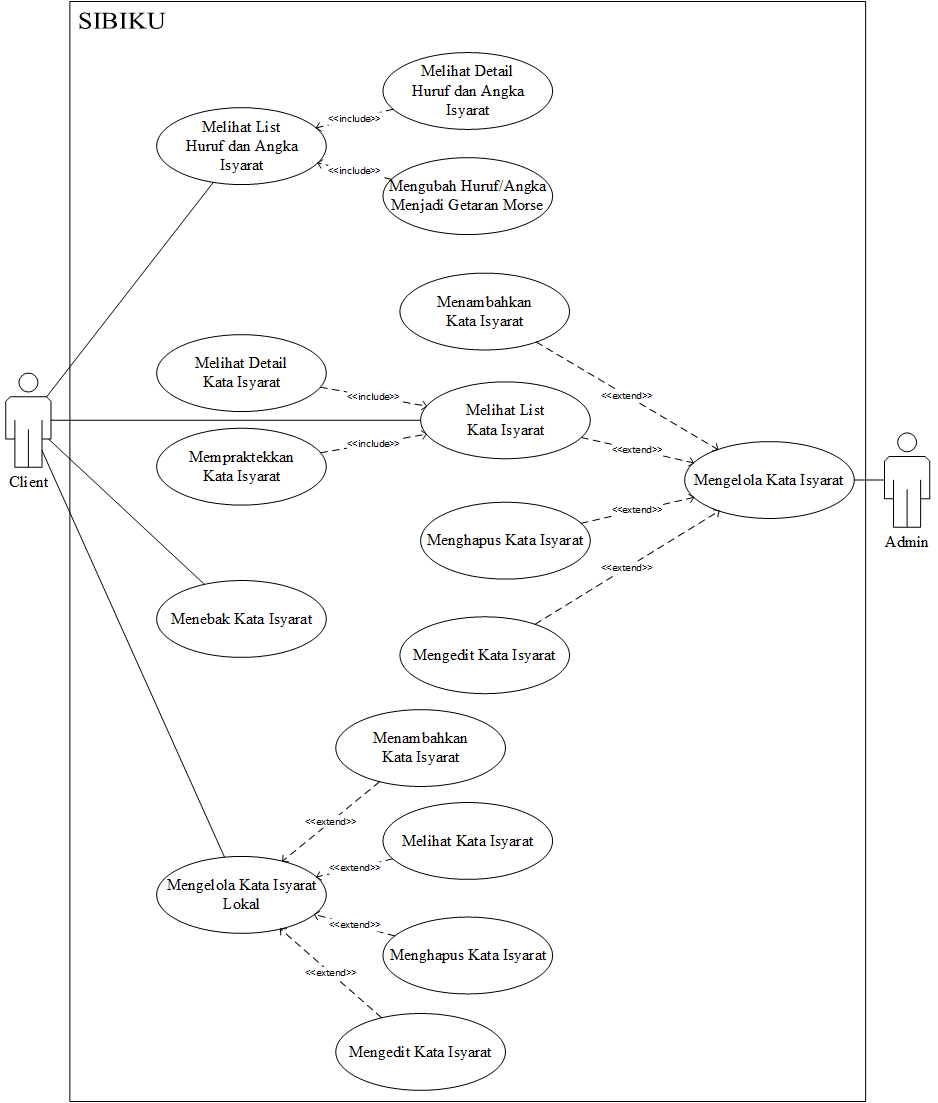
\includegraphics[height=8cm]{use-case-diagram}
    \caption{Use Case Diagram}
    \label{fig:usecase}
\end{figure}

Lorem ipsum dolor sit amet, consectetur adipiscing elit. Proin in porttitor
augue, vitae accumsan purus. Class aptent taciti sociosqu ad litora torquent per
conubia nostra, per inceptos himenaeos. Etiam pulvinar cursus magna vel eleifend.
Nunc gravida elit sed lectus accumsan tempus. Fusce et convallis magna, at
viverra ligula. Praesent rhoncus venenatis mattis. Sed maximus tortor tortor.

Curabitur id ullamcorper risus. Mauris in gravida libero, a lacinia ligula.
Donec consectetur purus non lectus eleifend, eu vehicula odio cursus.
Suspendisse potenti. Quisque quis erat in nunc fermentum fringilla quis eget
dui.

\subsection{Perancangan Antarmuka Aplikasi}
Bagian ini berisi rancangan antarmuka aplikasi berdasarkan analisis kebutuhan
pengguna dan use case diagram. Setiap rancangan tampilan wajib diberi penjelasan
berupa narasi apa yang dapat dilakukan pengguna di tampilan tersebut. Sehingga
pembaca dapat membayangkan seperti apa jalannya aplikasi nanti. Gunakan halaman
secara maksimal, jangan sampai muncul banyak spasi kosong.

Terdapat dua kemungkinan layout. Untuk tampilan potrait, penjelasan diletakkan
di samping gambar. Sedangkan untuk tampilan landscape, penjelasan diletakkan di
bawah gambar. Jika tabel berpindah halaman, pastikan judul kolom tabel juga ada
di halaman baru tersebut. Petunjuk: di Microsoft Word bisa klik Table layout,
kemudian aktifkan repeat header rows. Ikuti contoh di bawah ini:

Antarmuka aplikasi yang dirancang dapat disajikan dalam
Tabel~\ref{tab:rancangan-antarmuka}. Rancangan ini dibuat dengan menggunakan
prototyping tool berbasis web Figma. Setiap rancangan tampilan ini telah dicek
kesesuaiannya dengan analisis kebutuhan pengguna di subbab 3.1.3 dan juga
use-case diagram yang ada di subbab 3.2.2.

\begin{table}[H]
    \caption{Rancangan Antarmuka Aplikasi}
    \label{tab:rancangan-antarmuka}
    \centering
    \footnotesize
    \begin{tabular}{|c|p{4cm}|p{6cm}|}
        \hline
        \textbf{No.} & \textbf{Tampilan} & \textbf{Penjelasan} \\ \hline
        1 & \centering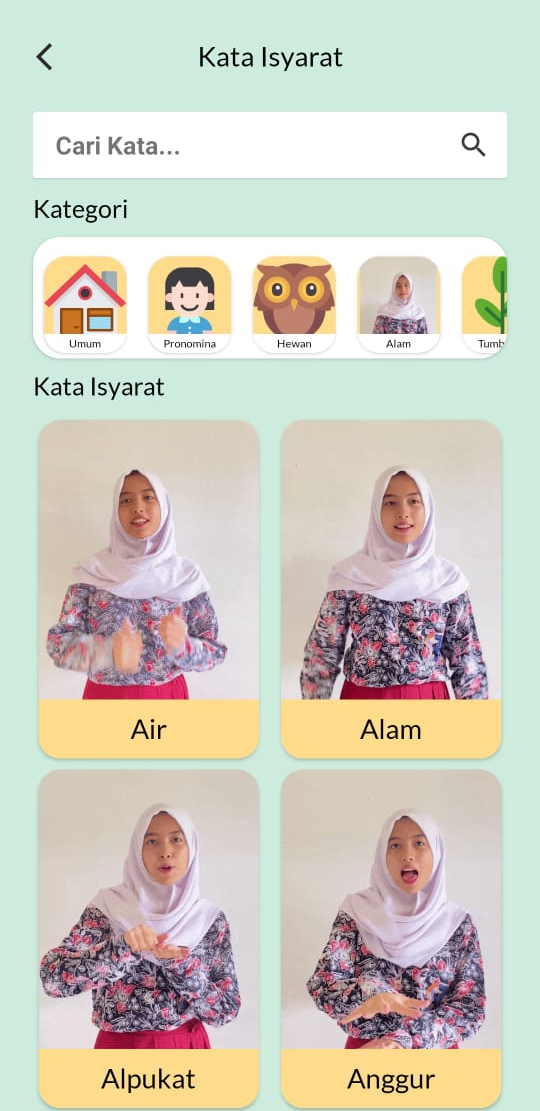
\includegraphics[height=4cm]{ui-kata-isyarat} & Tampilan ini muncul ketika pengguna melakukan klik pada menu Kata Isyarat. Di tampilan ini pengguna dapat melihat daftar kata isyarat yang diurutkan secara alfabetis. Jika pengguna melakukan klik pada salah satu kategori, maka kata isyarat yang muncul akan di-filter sesuai kategori yang dipilih. Selain itu pengguna juga dapat melakukan pencarian kata. Jika pengguna melakukan klik salah satu kata isyarat, maka akan muncul tampilan detil kata tersebut. \\ \hline
        2 & \centering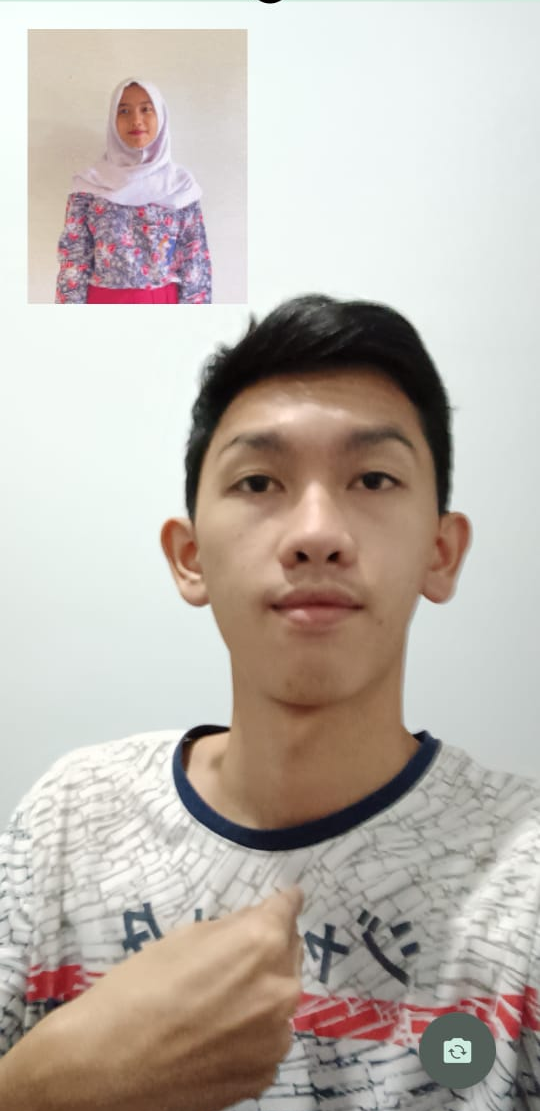
\includegraphics[height=4cm]{ui-nama-tampilan} & Lorem ipsum dolor sit amet, consectetur adipiscing elit. Proin in porttitor augue, vitae accumsan purus. Class aptent taciti sociosqu ad litora torquent per conubia nostra, per inceptos himenaeos. Etiam pulvinar cursus magna vel eleifend. Nunc gravida elit sed lectus accumsan tempus. Fusce et convallis magna, at viverra ligula. Praesent rhoncus venenatis mattis. Sed maximus tortor tortor. \\ \hline
    \end{tabular}
\end{table}

\subsection{Perancangan Basis Data}
Bagian ini berisi rancangan struktur data untuk menyimpan data yang diperlukan
aplikasi. Jika memakai database relasional seperti MySQL/SQLite, gunakan ERD.
Jika memakai database non-relasional, gunakan struktur tree. Jika tidak
menggunakan database, tetap wajib menuliskan strategi penyimpanan data, misal
menggunakan file dengan format tertentu, key-value pair, dan lain-lain. Contoh:

Untuk mendukung jalannya aplikasi, akan digunakan Firebase Realtime Database
dengan struktur data seperti tampak pada Gambar~\ref{fig:struktur-firebase}.

\begin{figure}[H]
    \centering
    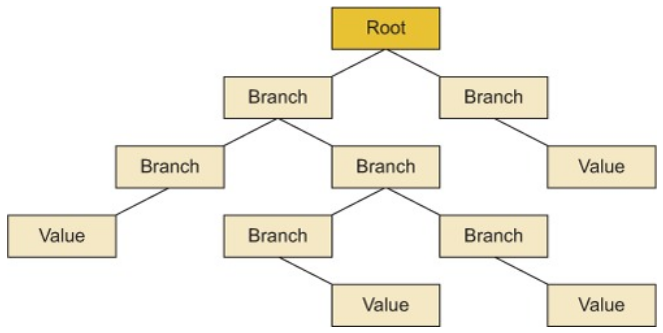
\includegraphics[width=0.85\textwidth]{struktur-firebase}
    \caption{Struktur Data Firebase Realtime Database}
    \label{fig:struktur-firebase}
\end{figure}

Selain itu, untuk kata isyarat lokal, aplikasi juga akan menggunakan database
SQLite dengan struktur data seperti Gambar~\ref{fig:struktur-sqlite}.

\begin{figure}[H]
    \centering
    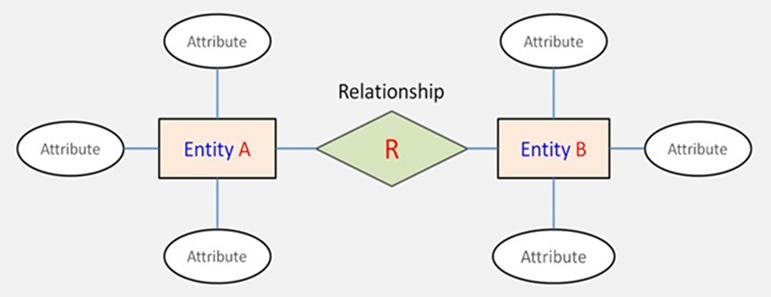
\includegraphics[width=0.8\textwidth]{struktur-sqlite}
    \caption{Struktur Data SQLite}
    \label{fig:struktur-sqlite}
\end{figure}

\subsection{Perancangan Perangkat IoT}
\textit{Bagian ini bersifat opsional dan hanya dibuat jika TA berbasis IoT yang
sensor-sensornya dirangkai sendiri menjadi sebuah perangkat.} Jelaskan sistematik
rangkaian perangkat IoT dan daftar hardware yang akan dipakai. Contoh:

Aplikasi yang dirancang membutuhkan sensor A, sensor B dan sensor C yang
disusun dalam sebuah rangkaian seperti Gambar~\ref{fig:skematik-iot}.

\begin{figure}[H]
    \centering
    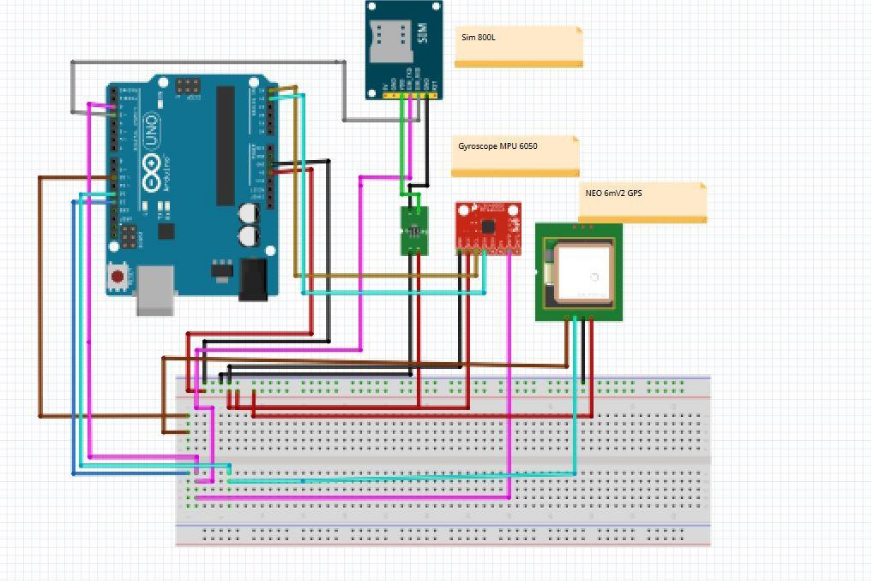
\includegraphics[width=0.5\textwidth]{skematik-iot}
    \caption{Rancangan Skematik Perangkat}
    \label{fig:skematik-iot}
\end{figure}

Hardware yang akan dipakai dalam perangkat beserta kegunaannya disajikan di
Tabel~\ref{tab:komponen-iot}.

\begin{table}[H]
    \caption{Daftar Komponen pada Perangkat}
    \label{tab:komponen-iot}
    \centering
    \begin{tabular}{|c|m{3.5cm}|c|m{4.5cm}|}
        \hline
        \textbf{No.} & \textbf{Komponen} & \textbf{Gambar} & \textbf{Penjelasan} \\ \hline
        1 & Arduino Uno & 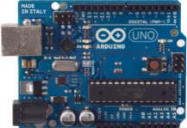
\includegraphics[height=3cm]{arduino-uno} & Untuk membuat berbagai hal yang berkaitan dengan fungsi mikrokontroler. \\ \hline
        2 & Gyroscope MPU6050 & 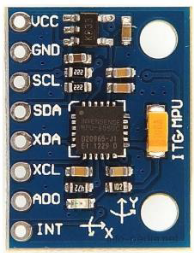
\includegraphics[height=4cm]{mpu6050} & Sensor ini bisa mendeteksi gerakan kemiringan sesuai gravitasi, sehingga bisa digunakan untuk mendeteksi gerakan pengguna. \\ \hline
    \end{tabular}
\end{table}

\noindent\textit{Catatan: gambar yang dipakai di tabel baiknya konsisten dengan
di rangkaian skematik, agar pembaca lebih mudah memahaminya.}

\section{Kebutuhan Pengembangan Aplikasi}
Untuk mengimplementasikan aplikasi sesuai rancangan yang telah dibuat, dibutuhkan
perangkat keras dan perangkat lunak berikut.

\subsection{Kebutuhan Perangkat Keras}
Perangkat keras yang dibutuhkan disajikan dalam Tabel~\ref{tab:kebutuhan-hw}.
Terdapat perangkat yang belum tersedia sehingga harus dibeli dengan total
estimasi biaya sebesar Rp.\ 1.500.000,-

\begin{table}[H]
    \caption{Kebutuhan Perangkat Keras}
    \label{tab:kebutuhan-hw}
    \centering
    \footnotesize
    \begin{tabular}{|c|p{6.5cm}|p{4cm}|}
        \hline
        \textbf{No.} & \textbf{Spesifikasi Perangkat} & \textbf{Ketersediaan} \\ \hline
        1 & Laptop Asus ROG GL503GE:\newline Intel Core\textsuperscript{TM} i7 dan RAM 8GB & Tersedia, milik pribadi \\ \hline
        2 & Smartphone Samsung A50:\newline layar 6.4'' dan RAM 4GB & Tersedia, milik pribadi \\ \hline
        3 & Oculus Quest 2 & Akan meminjam dari lab \\ \hline
        4 & Arduino Uno & Akan dibeli, harga Rp.\ 90.000 \\ \hline
        5 & Gyroscope MPU6050 & Akan dibeli, harga Rp.\ 45.000 \\ \hline
        \ldots & \ldots & \ldots \\ \hline
        dst & dst & dst \\ \hline
    \end{tabular}
\end{table}

\subsection{Kebutuhan Perangkat Lunak}
Perangkat lunak yang dibutuhkan disajikan dalam Tabel~\ref{tab:kebutuhan-sw}.
Semua perangkat lunak yang akan digunakan berlisensi dan dijamin bukan bajakan.
Tidak terdapat biaya yang harus dibayarkan untuk mendapatkan perangkat lunak
yang dibutuhkan.

\begin{table}[H]
    \caption{Kebutuhan Perangkat Lunak}
    \label{tab:kebutuhan-sw}
    \centering
    \begin{tabular}{|c|p{6.5cm}|p{4cm}|}
        \hline
        \textbf{No.} & \textbf{Spesifikasi Perangkat} & \textbf{Lisensi} \\ \hline
        1 & Android Studio Arctic Fox - 2020.3.1 & Open source \\ \hline
        2 & Firebase Realtime Database & Spark plan (free) \\ \hline
        3 & Firebase Cloud Storage & Spark plan (free) \\ \hline
        4 & Unity 2020.3 & Personal license \\ \hline
        5 & Arduino IDE & Open source \\ \hline
        \ldots & \ldots & \ldots \\ \hline
        dst & dst & dst \\ \hline
    \end{tabular}
\end{table}

% =====================================================================
% BAB IV IMPLEMENTASI DAN PENGUJIAN
% =====================================================================
\chapter{Implementasi dan Pengujian}

\section{Implementasi Aplikasi}
Implementasi dilakukan berdasarkan rancangan yang telah dibuat di bab
sebelumnya. Struktur kode project, kesesuaian antara rancangan dengan
implementasi serta hasil implementasi dapat dibahas sebagai berikut.

\subsection{Struktur Kode Project}
Bagian ini berisi penjelasan mengenai struktur kode yang digunakan dalam
project. Termasuk juga teknik coding, pendekatan, arsitektur atau hal lain yang
relevan. Buatlah agar pembaca mengerti bagaimana project ini disusun.

Seperti telah dijelaskan di subbab 3.2.1, aplikasi SIBIKU terdiri dari dua
bagian, yaitu aplikasi siswa dan aplikasi guru/admin. Ini diimplementasikan di
Android Studio dengan menggunakan pendekatan single project multiple modules.
Dengan cara ini, source code akan lebih mudah di-maintain, karena kode kedua
aplikasi berada di project yang sama. Struktur kode project ditunjukkan pada
Gambar~\ref{fig:struktur-kode}.

\begin{figure}[H]
    \centering
    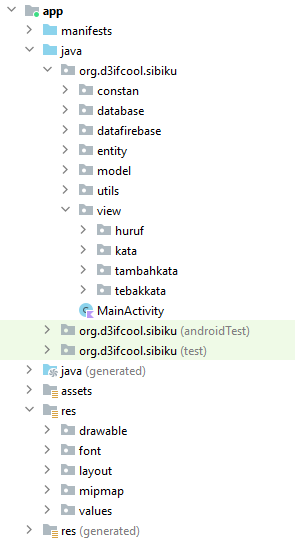
\includegraphics[height=9cm]{struktur-kode-1}\hspace{0.3cm}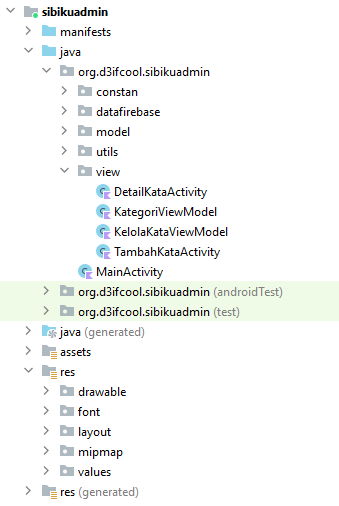
\includegraphics[height=4.5cm]{struktur-kode-2}
    \caption{Struktur Kode Project}
    \label{fig:struktur-kode}
\end{figure}

Selain itu, implementasi juga dilakukan dengan arsitektur MVVM yang memisahkan
kode terkait UI dengan kode terkait business logic aplikasi. Kelas-kelas yang
ada juga dibagi ke dalam package-package sesuai fungsinya masing-masing.
Penamaan package, kelas dan nama variabel telah dibuat sesuai konvensi yang
berlaku umum sehingga tidak perlu dijelaskan lagi secara detail satu per satu.

Sesuai dengan best practice di industri, project ini juga telah menerapkan
version control system (VCS) sehingga setiap perubahan pada kode akan tersimpan
riwayatnya. VCS yang digunakan adalah git, dan project di-hosting di Github
untuk memudahkan kolaborasi dalam tim. Repositori bersifat private dan dapat
diakses di link berikut jika diperlukan:
\url{https://github.com/PA-IZM/42-kamus-sibi}

\subsection{Kesesuaian Terhadap Rancangan}
Rencana berubah itu biasa. Uraikan kesesuaian antara rancangan dengan
implementasi yang kalian lakukan. Untuk setiap perubahan, ceritakan apa yang
berubah dan kenapa? Ini akan memberi tahu pembaca story pengerjaan tugas akhir
ini. Ceritakan juga kendala yang dihadapi ketika proses implementasi. Kendala
boleh yang bersifat teknis maupun non-teknis. Perhatikan contoh berikut ini:

Oleh karena proses perancangan telah melibatkan berbagai pihak mulai dari dosen
pembimbing, dosen reviewer hingga calon pengguna, dalam hal ini guru, siswa dan
orang tua siswa SLBN Cicendo Bandung, tidak ada perubahan yang signifikan di
aplikasi hasil implementasi. Semua fitur maupun fungsionalitas tetap sama dengan
rancangan Bab III. Hanya terdapat sedikit perbedaan saja di UI.

Sebagai contoh, pada tampilan huruf dan angka, pada awalnya kode morse baru akan
muncul setelah huruf atau angka tersebut diklik. Setelah diimplementasikan, baru
terasa bahwa akan jadi lebih baik jika kode morse dapat langsung dilihat oleh
pengguna di tampilan list. Masih di tampilan ini, karena pada saat perancangan
aset yang tersedia terbatas, terdapat aset yang berlatar putih. Ini telah
diperbaiki saat implementasi sehingga tampilan menjadi lebih konsisten.

\begin{figure}[H]
    \centering
    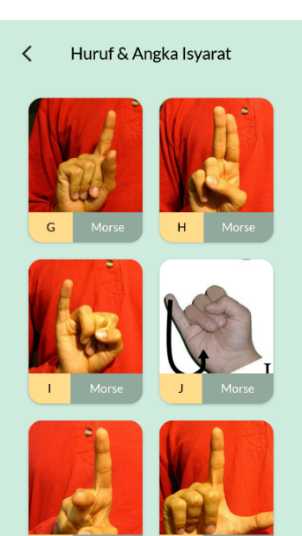
\includegraphics[height=7cm]{perbedaan-ui-1}\hspace{0.3cm}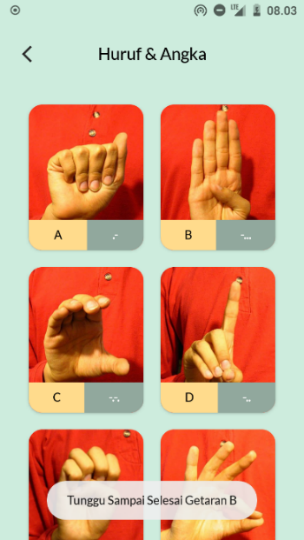
\includegraphics[height=7cm]{perbedaan-ui-2}
    \caption{Perbedaan UI Rancangan dan Implementasi}
    \label{fig:perbedaan-ui}
\end{figure}

Perbedaan lainnya adalah pada tampilan lorem ipsum dolor sit amet, consectetur
adipiscing elit. Proin in porttitor augue, vitae accumsan purus. Class aptent
taciti sociosqu ad litora torquent per conubia nostra, per inceptos himenaeos.
Etiam pulvinar cursus magna vel eleifend. Nunc gravida elit sed lectus accumsan
tempus. Fusce et convallis magna, at viverra ligula praesent rhoncus.

Curabitur id ullamcorper risus. Mauris in gravida libero, a lacinia ligula.
Donec consectetur purus non lectus eleifend, eu vehicula odio cursus.
Suspendisse potenti. Quisque quis erat in nunc fermentum fringilla quis eget
dui. Donec tortor odio, tincidunt ac faucibus eget, elementum eget massa. Sed ac
ante ac nulla maximus lobortis a vel dui. Pellentesque pellentesque in orci id
finibus.

Dari sisi database, terdapat sedikit modifikasi pada struktur Firebase Realtime
Database. Perubahan dilakukan pada ID kata isyarat, dimana awalnya ID bertipe
number karena rencananya akan menggunakan auto increment sebagaimana di
database SQLite. Saat implementasi, ternyata ada kelemahan pada skema tersebut.
Terjadi race condition ketika admin menggunakan lebih dari satu device secara
bersamaan. Akhirnya ID diubah menjadi bertipe string dan menggunakan key yang
di-generate oleh Firebase. Dengan demikian masalah tersebut dapat diatasi.

Ketika melakukan implementasi aplikasi, tidak ada kendala yang berarti dari sisi
teknis pemrograman, sebab hal-hal yang dipakai di tugas akhir ini telah
diajarkan di mata kuliah. Hanya saja, beberapa hal seperti perubahan UI/UX dan
struktur database seperti di atas baru terpikirkan setelah rancangan
diimplementasikan. Dari sisi non-teknis, ternyata menyiapkan aset kata isyarat
lumayan menyita waktu, mulai dari proses shooting, editing hingga input ke
aplikasi.

\subsection{Hasil Implementasi}
Bagian ini berisi penjelasan mengenai hasil implementasi tugas akhir ini berupa
apa, dan bisa diakses dimana. Gunakan folder Google Drive yang diberikan oleh
prodi. Gunakan juga URL shortener karena link asli Google Drive cukup panjang,
dan sulit diketik manual.

Jika tidak ada perbedaan yang signifikan antara aplikasi hasil implementasi
dengan rancangannya, maka tidak perlu menampilkan screenshot aplikasi jadi,
karena sudah tercover di subbab 3.2.3.

Hasil implementasi tugas akhir ini ada dua, yaitu aplikasi siswa dan aplikasi
guru/admin. Kedua aplikasi tersebut tersedia dalam bentuk berkas APK dan dapat
diunduh dari tautan berikut menggunakan email Tel-U. Untuk mempermudah
pengoperasian aplikasi, pada tautan tersebut juga terdapat buku panduan
penggunaan aplikasi, video demo aplikasi, video promosi aplikasi serta poster:
\url{https://tel-u.ac.id/artefak-sibiku}

\section{Pengujian Aplikasi}
Untuk memastikan kualitasnya, aplikasi ini diuji dalam 3 tahapan, mulai dari
kualitas kode, pengujian fungsionalitas hingga pengujian ke pengguna.

\subsection{Pengujian Kualitas Kode}
Jelaskan cara yang ditempuh untuk memastikan bahwa kode yang ditulis telah
memenuhi kualitas kode yang baik. Akan lebih bagus jika disajikan data
kuantitatif seperti jumlah warning ketika pengujian awal dan pengujian akhir.
Berikan justifikasi jika ada hal-hal yang tidak ditangani atau diabaikan. Contoh:

Pengujian kualitas kode project dilakukan dengan menggunakan tools Inspect Code
yang disediakan oleh Android Studio. Pada awalnya terdapat 201 warning dan 21
weak warning. Setelah dilakukan perbaikan, tersisa 9 warning dan 3 weak warning
seperti ditunjukkan pada Gambar~\ref{fig:inspect-code}. Warning ini tidak bersifat
material dan dapat diabaikan. Terdapat 4.149 typo yang merupakan false positive
dikarenakan penggunaan Bahasa Indonesia di kode aplikasi sehingga dapat
diabaikan juga.

\begin{figure}[H]
    \centering
    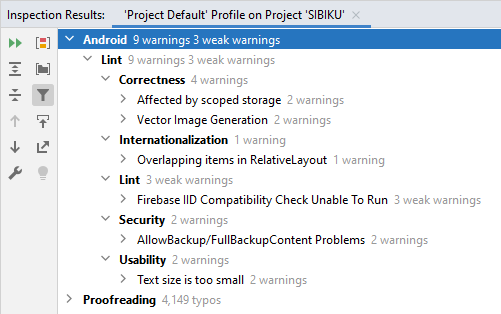
\includegraphics[width=0.8\textwidth]{inspect-code}
    \caption{Hasil Inspect Code}
    \label{fig:inspect-code}
\end{figure}

Lorem ipsum dolor sit amet, consectetur adipiscing elit. Proin in porttitor
augue, vitae accumsan purus. Class aptent taciti sociosqu ad litora torquent per
conubia nostra, per inceptos himenaeos. Etiam pulvinar cursus magna vel eleifend.
Nunc gravida elit sed lectus accumsan tempus. Fusce et convallis magna, at
viverra ligula. Praesent rhoncus venenatis mattis. Sed maximus tortor tortor.

Curabitur id ullamcorper risus. Mauris in gravida libero, a lacinia ligula.
Donec consectetur purus non lectus eleifend, eu vehicula odio cursus.
Suspendisse potenti. Quisque quis erat in nunc fermentum fringilla quis eget
dui. Donec tortor odio, tincidunt ac faucibus eget, elementum eget massa. Sed ac
ante ac nulla maximus lobortis a vel dui. Pellentesque pellentesque in orci id
finibus.

\subsection{Pengujian Fungsionalitas}
Jelaskan metode pengujian yang dilakukan untuk menguji fungsionalitas aplikasi,
serta perangkat yang digunakan ketika melakukan pengujian. Test yang sifatnya
tidak material seperti pengujian splashscreen dan about boleh tidak ditulis.
Tutup subbab ini dengan kesimpulan hasil pengujian fungsionalitas. Contoh:

Uji fungsionalitas aplikasi dilakukan dengan metode black box. Pengujian diawali
dengan membuat skenario test untuk setiap fitur aplikasi, lalu menerjemahkan
skenario tersebut ke dalam instrumentation test menggunakan Espresso. Seluruh
pengujian aplikasi ini dilakukan menggunakan smartphone Redmi Note 10S dan
sistem operasi Android 11. Berikut rincian test yang dilakukan beserta hasilnya.

\begin{table}[H]
    \caption{Detail Pengujian Fungsionalitas (contoh: 1.a)}
    \label{tab:detail-test}
    \centering
    \footnotesize
    \begin{tabular}{|p{3cm}|p{10cm}|}
        \hline
        \textbf{Nomor Tes} & 1.a \\ \hline
        \textbf{Judul} & Menguji fungsionalitas huruf beserta morse \\ \hline
        \textbf{Teknik} & \begin{minipage}{\linewidth}
\begin{lstlisting}[basicstyle=\ttfamily\scriptsize,frame=none]
@Test
fun listHurufTestActivity() {
    val rvMenu = onView(withId(R.id.rvMenu))
    rvMenu.perform(actionOnItemAtPosition
            <ViewHolder>(0, click()))
    Thread.sleep(4000)
    val rvHuruf = onView(withId(R.id.rv_huruf))
    rvHuruf.perform(actionOnItemAtPosition
            <ViewHolder>(0, click()))
    val huruf = onView(withId(R.id.tvDetailHuruf))
    huruf.check(ViewAssertions.matches
            (withText(HURUF_PILIHAN)))
}
\end{lstlisting}
\textit{Noted: Penulisan Source Code menggunakan font Consolas ukuran 10}
\end{minipage} \\ \hline
        \textbf{Kriteria Keberhasilan} & Ketika klik menu huruf dan angka pada tampilan utama, muncul tampilan list huruf. Ketika salah satu huruf diklik, muncul informasi detail dari huruf tersebut. \\ \hline
        \textbf{Hasil} & 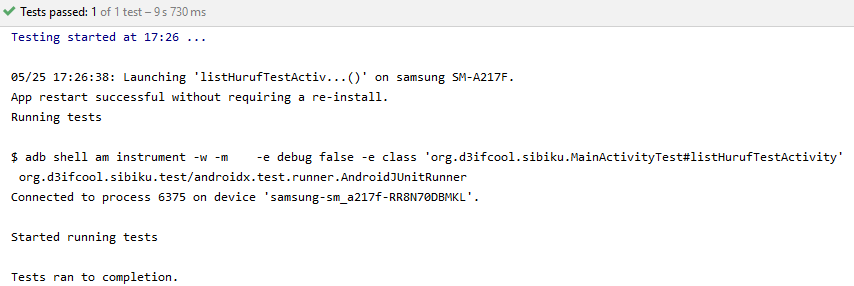
\includegraphics[width=0.7\linewidth]{test-hasil} \\ \hline
    \end{tabular}
\end{table}

\noindent Berdasarkan pengujian-pengujian yang telah dilakukan di atas, dapat
disimpulkan bahwa fitur-fitur di dalam aplikasi yang dikembangkan telah berjalan
dengan baik dan hasil yang didapat telah sesuai dengan yang diharapkan.

\subsection{Pengujian ke Pengguna}
Jelaskan metode pengujian yang dilakukan ke pengguna beserta tahapan-tahapannya.
Tuliskan data responden yang terlibat dalam pengujian, serta hasil pengujiannya
seperti apa. Jangan lupa untuk melampirkan dokumentasi pengujian di lampiran A
dan detail perhitungan hasil pengujian di lampiran B.

Pengujian ke pengguna dilakukan dengan metode usability test. Proses pengujian
diawali dengan membuat kuesioner di Google Form, lalu menyebarkan kuesioner
tersebut ke responden. Selanjutnya, dilakukan perhitungan hasil kuesioner dengan
skala Likert. Terakhir, dilakukan interpretasi hasil perhitungan.

Pengujian dilakukan dengan responden sebanyak 71 orang terdiri dari 35,2\% siswa
SLB, 12,7\% dosen/guru, 45,1\% mahasiswa, dan 7\% lainnya. Setiap responden
dipastikan telah mencoba aplikasi sebelum mengisi kuesioner, sebab pengujian
dilakukan secara sinkron melalui aplikasi Zoom. Dokumentasi kegiatan dapat
dilihat di lampiran A, dan daftar pertanyaan yang diajukan serta perhitungan
hasil kuesioner dapat dilihat di lampiran B.

Berdasarkan hasil perhitungan, sebanyak 89,7\% responden sangat setuju aplikasi
telah berhasil menerapkan effectiveness dalam fitur-fiturnya, seperti terlihat
pada Gambar~\ref{fig:grafik-effectiveness}.

\begin{figure}[H]
    \centering
    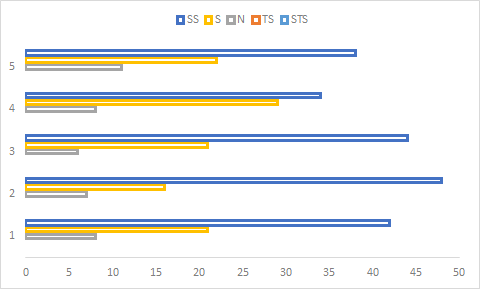
\includegraphics[width=0.8\textwidth]{grafik-effectiveness}
    \caption{Grafik Respon Effectiveness}
    \label{fig:grafik-effectiveness}
\end{figure}

Lorem ipsum dolor sit amet, consectetur adipiscing elit. Proin in porttitor
augue, vitae accumsan purus. Class aptent taciti sociosqu ad litora torquent per
conubia nostra, per inceptos himenaeos. Etiam pulvinar cursus magna vel
eleifend. Nunc gravida elit sed lectus accumsan tempus. Fusce et convallis magna.
At viverra ligula. Praesent rhoncus venenatis mattis. Sed maximus tortor tortor.
Curabitur id ullamcorper risus. Mauris in gravida libero, a lacinia ligula.
Donec consectetur purus non lectus eleifend, eu vehicula odio cursus.

\subsection{Diskusi Hasil Pengujian}
Bagian ini berisi interpretasi hasil pengujian yang telah dilakukan, dikaitkan
dengan rumusan masalah dan tujuan tugas akhir yang ada di Bab 1. Sebagai contoh,
jika tujuan TA ini adalah X, pengujian manakah yang mendukung tujuan tersebut
sehingga dapat dikatakan tujuan TA ini telah tercapai?

Lorem ipsum dolor sit amet, consectetur adipiscing elit. Morbi sed lacus orci.
Aliquam cursus faucibus orci, eu sodales dolor pulvinar at. Integer maximus augue
at magna lacinia cursus. Class aptent taciti sociosqu ad litora torquent per
conubia nostra, per inceptos himenaeos. Aenean quis feugiat lorem. Sed iaculis
varius congue. Fusce posuere euismod ante, a ornare ex consequat sit amet.

Proin ac tellus ipsum. Sed congue imperdiet feugiat. Sed mattis blandit risus,
et blandit est pulvinar vel. Donec aliquet est id dolor consectetur ultrices.
Orci varius natoque penatibus et magnis dis parturient montes, nascitur
ridiculus mus.

% =====================================================================
% BAB V KESIMPULAN DAN SARAN
% =====================================================================
\chapter{Kesimpulan dan Saran}

\section{Kesimpulan}
Bagian ini berisi kesimpulan yang didapat setelah implementasi aplikasi dan
pengujian ke pengguna. Kesimpulan sedapatnya harus sesuai dengan rumusan masalah
dan tujuan dibuatnya tugas akhir ini di Bab 1. Contoh:

Berdasarkan aplikasi yang telah dibangun dan pengujian yang telah dilakukan,
dapat disimpulkan bahwa aplikasi SIBIKU merupakan media belajar yang bagus dan
dapat membantu siswa SLB penyandang tunarungu dalam belajar bahasa isyarat
dengan mudah. Selain itu, aplikasi ini juga dapat membantu sekolah dan guru
dalam pembelajaran kosakata baru pada siswa SLB.

Dengan demikian, aplikasi SIBIKU telah berhasil mencapai tujuannya. Ini
dibuktikan pada pengujian ke pengguna yang melibatkan 71 responden, dimana
91,30\% pengguna sangat setuju bahwa aplikasi SIBIKU sangat efektif sebagai media
dalam kegiatan belajar pada siswa SLB penyandang tunarungu, berkat fitur tebak
kata yang meningkatkan semangat belajar dan juga sebagai evaluasi mandiri.

\section{Saran}
Tidak ada aplikasi yang sempurna. Isi bagian ini dengan hal-hal yang dapat
membuat aplikasi kalian menjadi lebih baik lagi. Boleh saran berupa penambahan
fitur baru, atau perbaikan fitur yang sudah ada. Dilarang memberikan saran yang
mengambang karena akan membuat pembaca jadi bingung.

Berdasarkan hasil pengujian yang dilakukan, berikut saran yang dapat diberikan
untuk pengembangan aplikasi lebih lanjut:
\begin{itemize}
    \item Kosakata isyarat lebih diperbanyak lagi.
    \item Penambahan filter kata isyarat berdasarkan kelas.
    \item Penambahan fitur ranking berdasarkan poin yang didapat dari keaktifan
    pengguna dalam menggunakan aplikasi SIBIKU.
    \item Aplikasi dibuat dalam platform iOS.
\end{itemize}

% =====================================================================
% DAFTAR PUSTAKA
% =====================================================================
\renewcommand{\bibname}{Daftar Pustaka}
\begin{thebibliography}{9}
\bibitem{ref1}
I. Tin, ``Liputan 6 Tekno,'' 21 November 2016. [Online]. Available:
\url{http://tekno.liputan6.com/read/2591339/tak-disangka-pengguna-bitcoin-di-indonesia-capai-200-ribu}.

\bibitem{ref2}
\textit{(Referensi kedua -- tulis sesuai format IEEE)}

\bibitem{ref3}
\textit{(Referensi ketiga -- tulis sesuai format IEEE)}

\bibitem{ref4}
\textit{(Referensi keempat -- tulis sesuai format IEEE)}

\bibitem{ref5}
\textit{(Referensi kelima -- tulis sesuai format IEEE)}
\end{thebibliography}

\noindent\textbf{Catatan:} Harap diingat bahwa masing-masing sumber yang anda
gunakan dan didapatkan dari manapun juga, harus ditulis didalam bagian daftar
pustaka ini. Demikian pula setiap item yang ada pada bagian daftar pustaka telah
pernah dirujuk dalam bab-bab sebelumnya.

% =====================================================================
% LAMPIRAN
% =====================================================================
\appendix

\chapter{Dokumentasi Kegiatan}
\label{sec:lampiran-dokumentasi}

\begin{figure}[H]
    \centering
    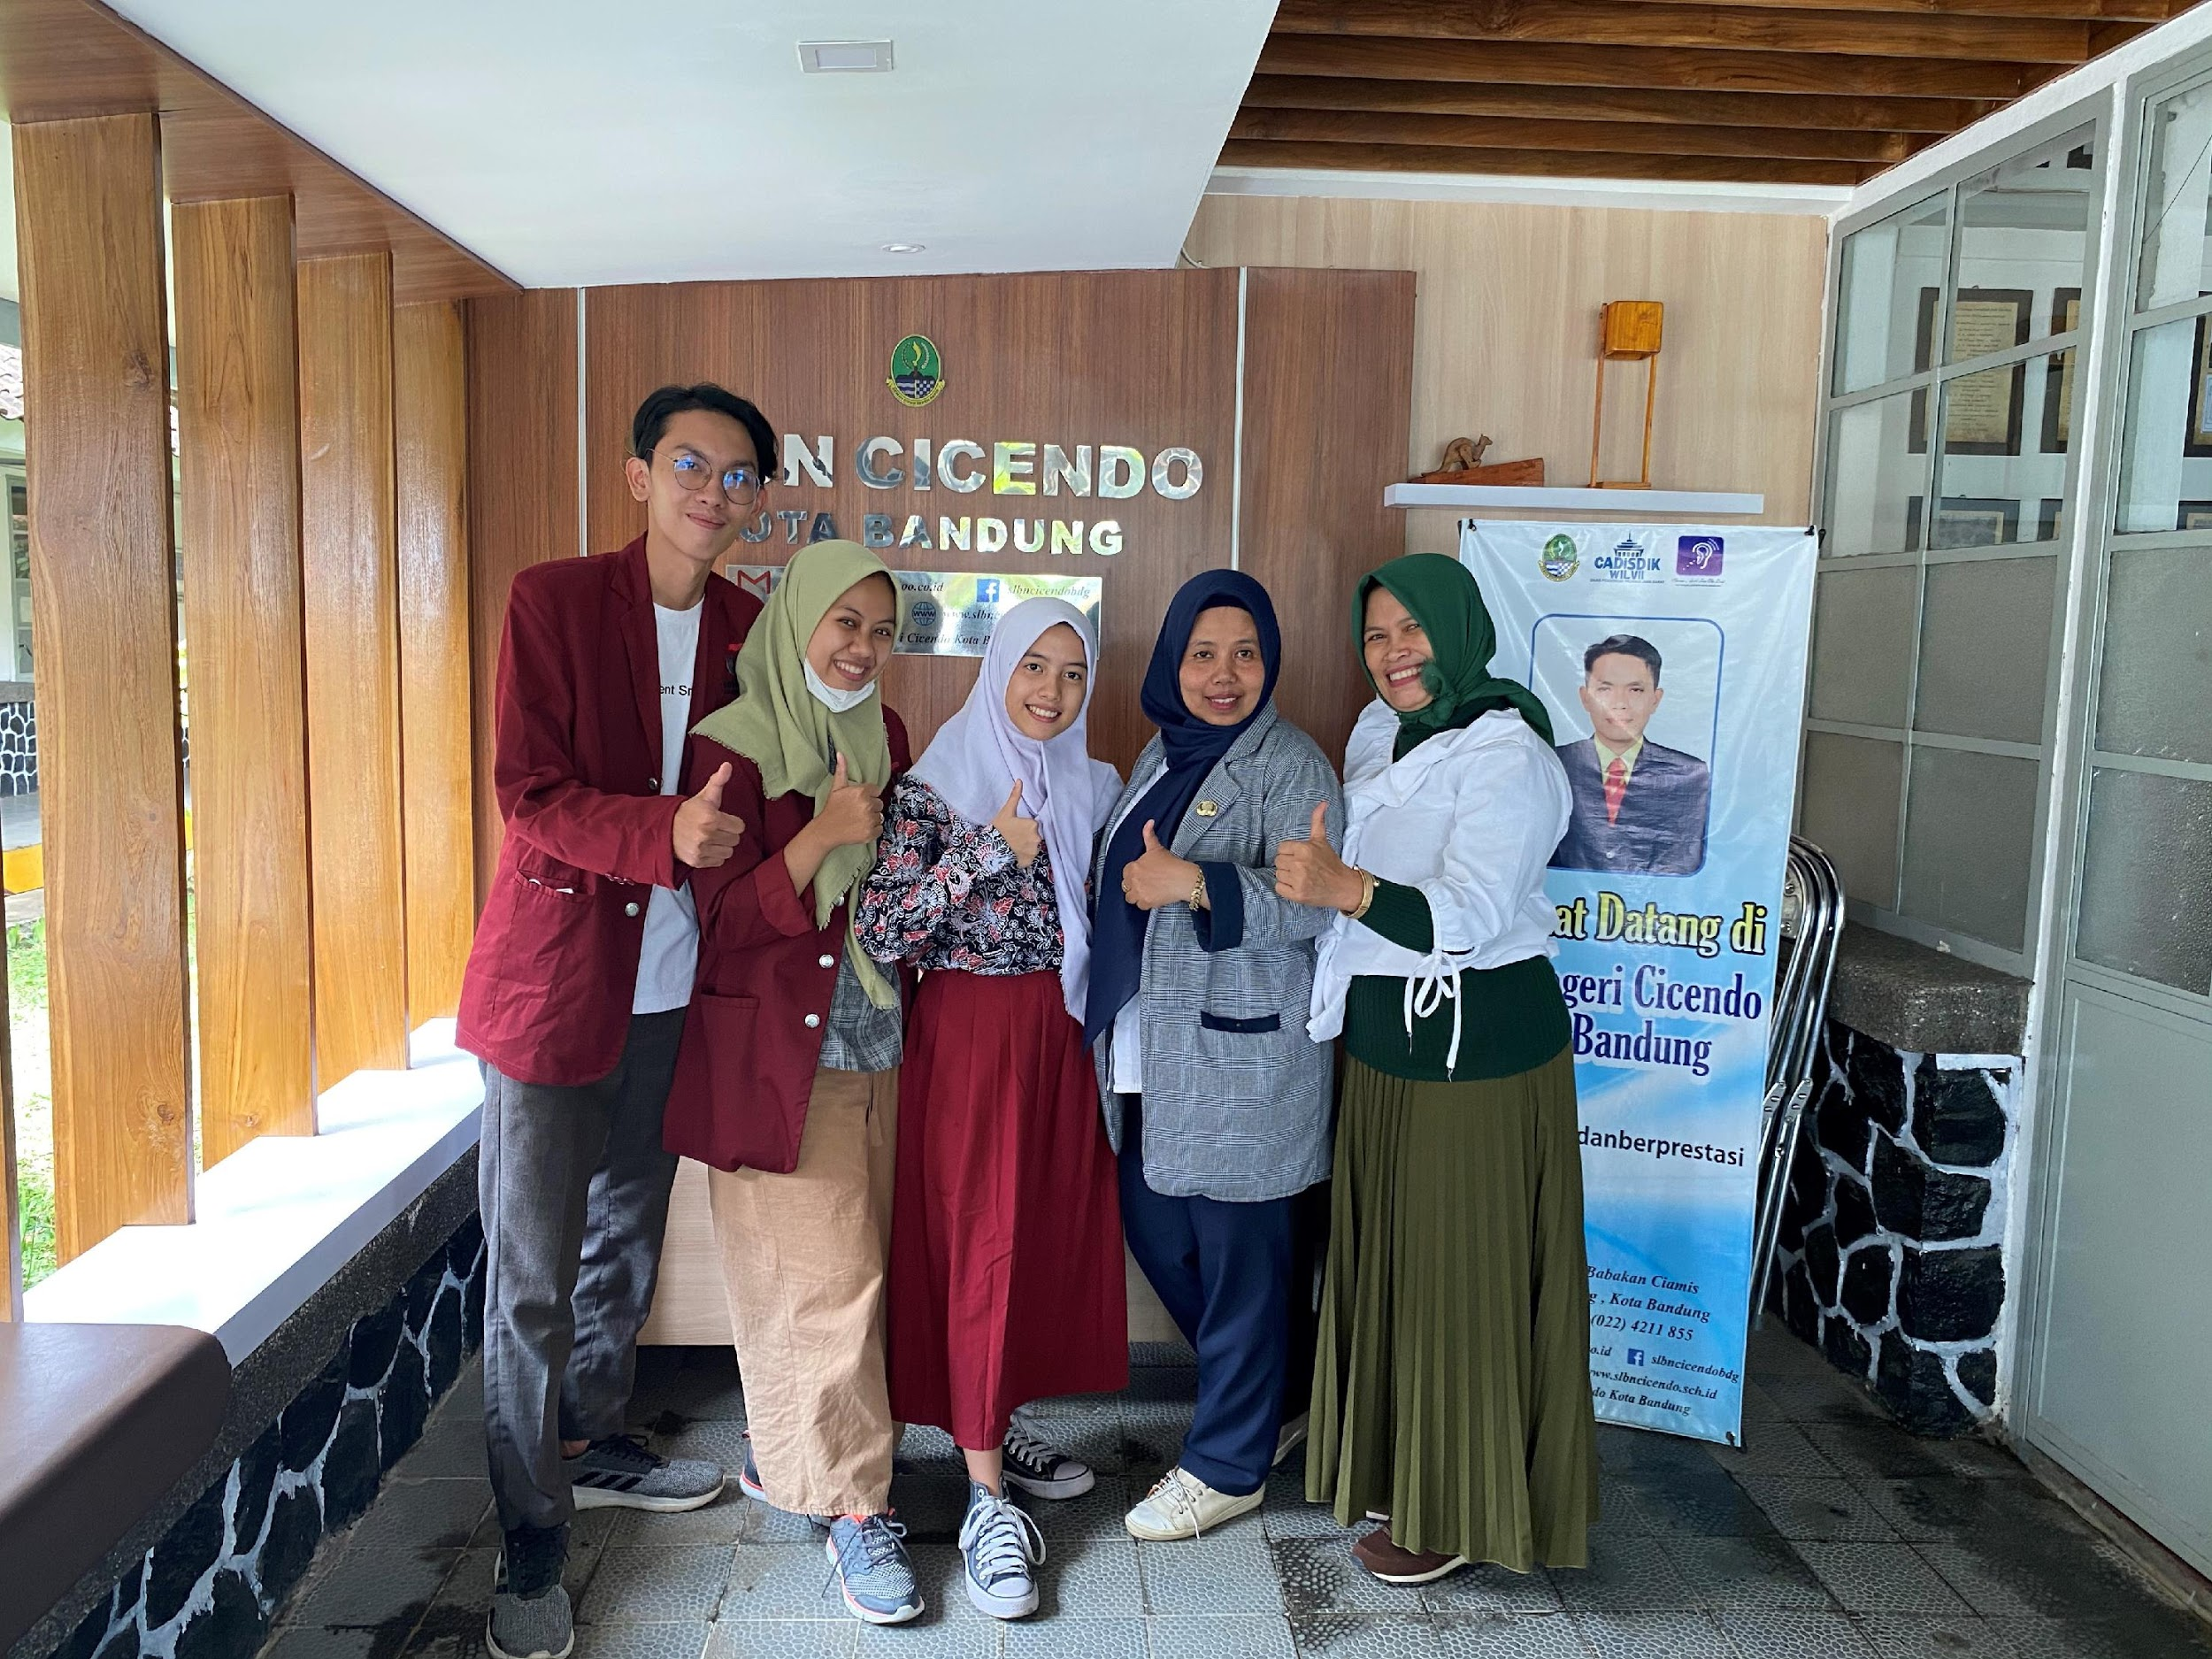
\includegraphics[width=0.8\textwidth]{lampiran-a-1}
    \caption{Foto bersama siswa yang diwawancarai dan dua orang gurunya.}
    \label{fig:lampiran-a-1}
\end{figure}

\begin{figure}[H]
    \centering
    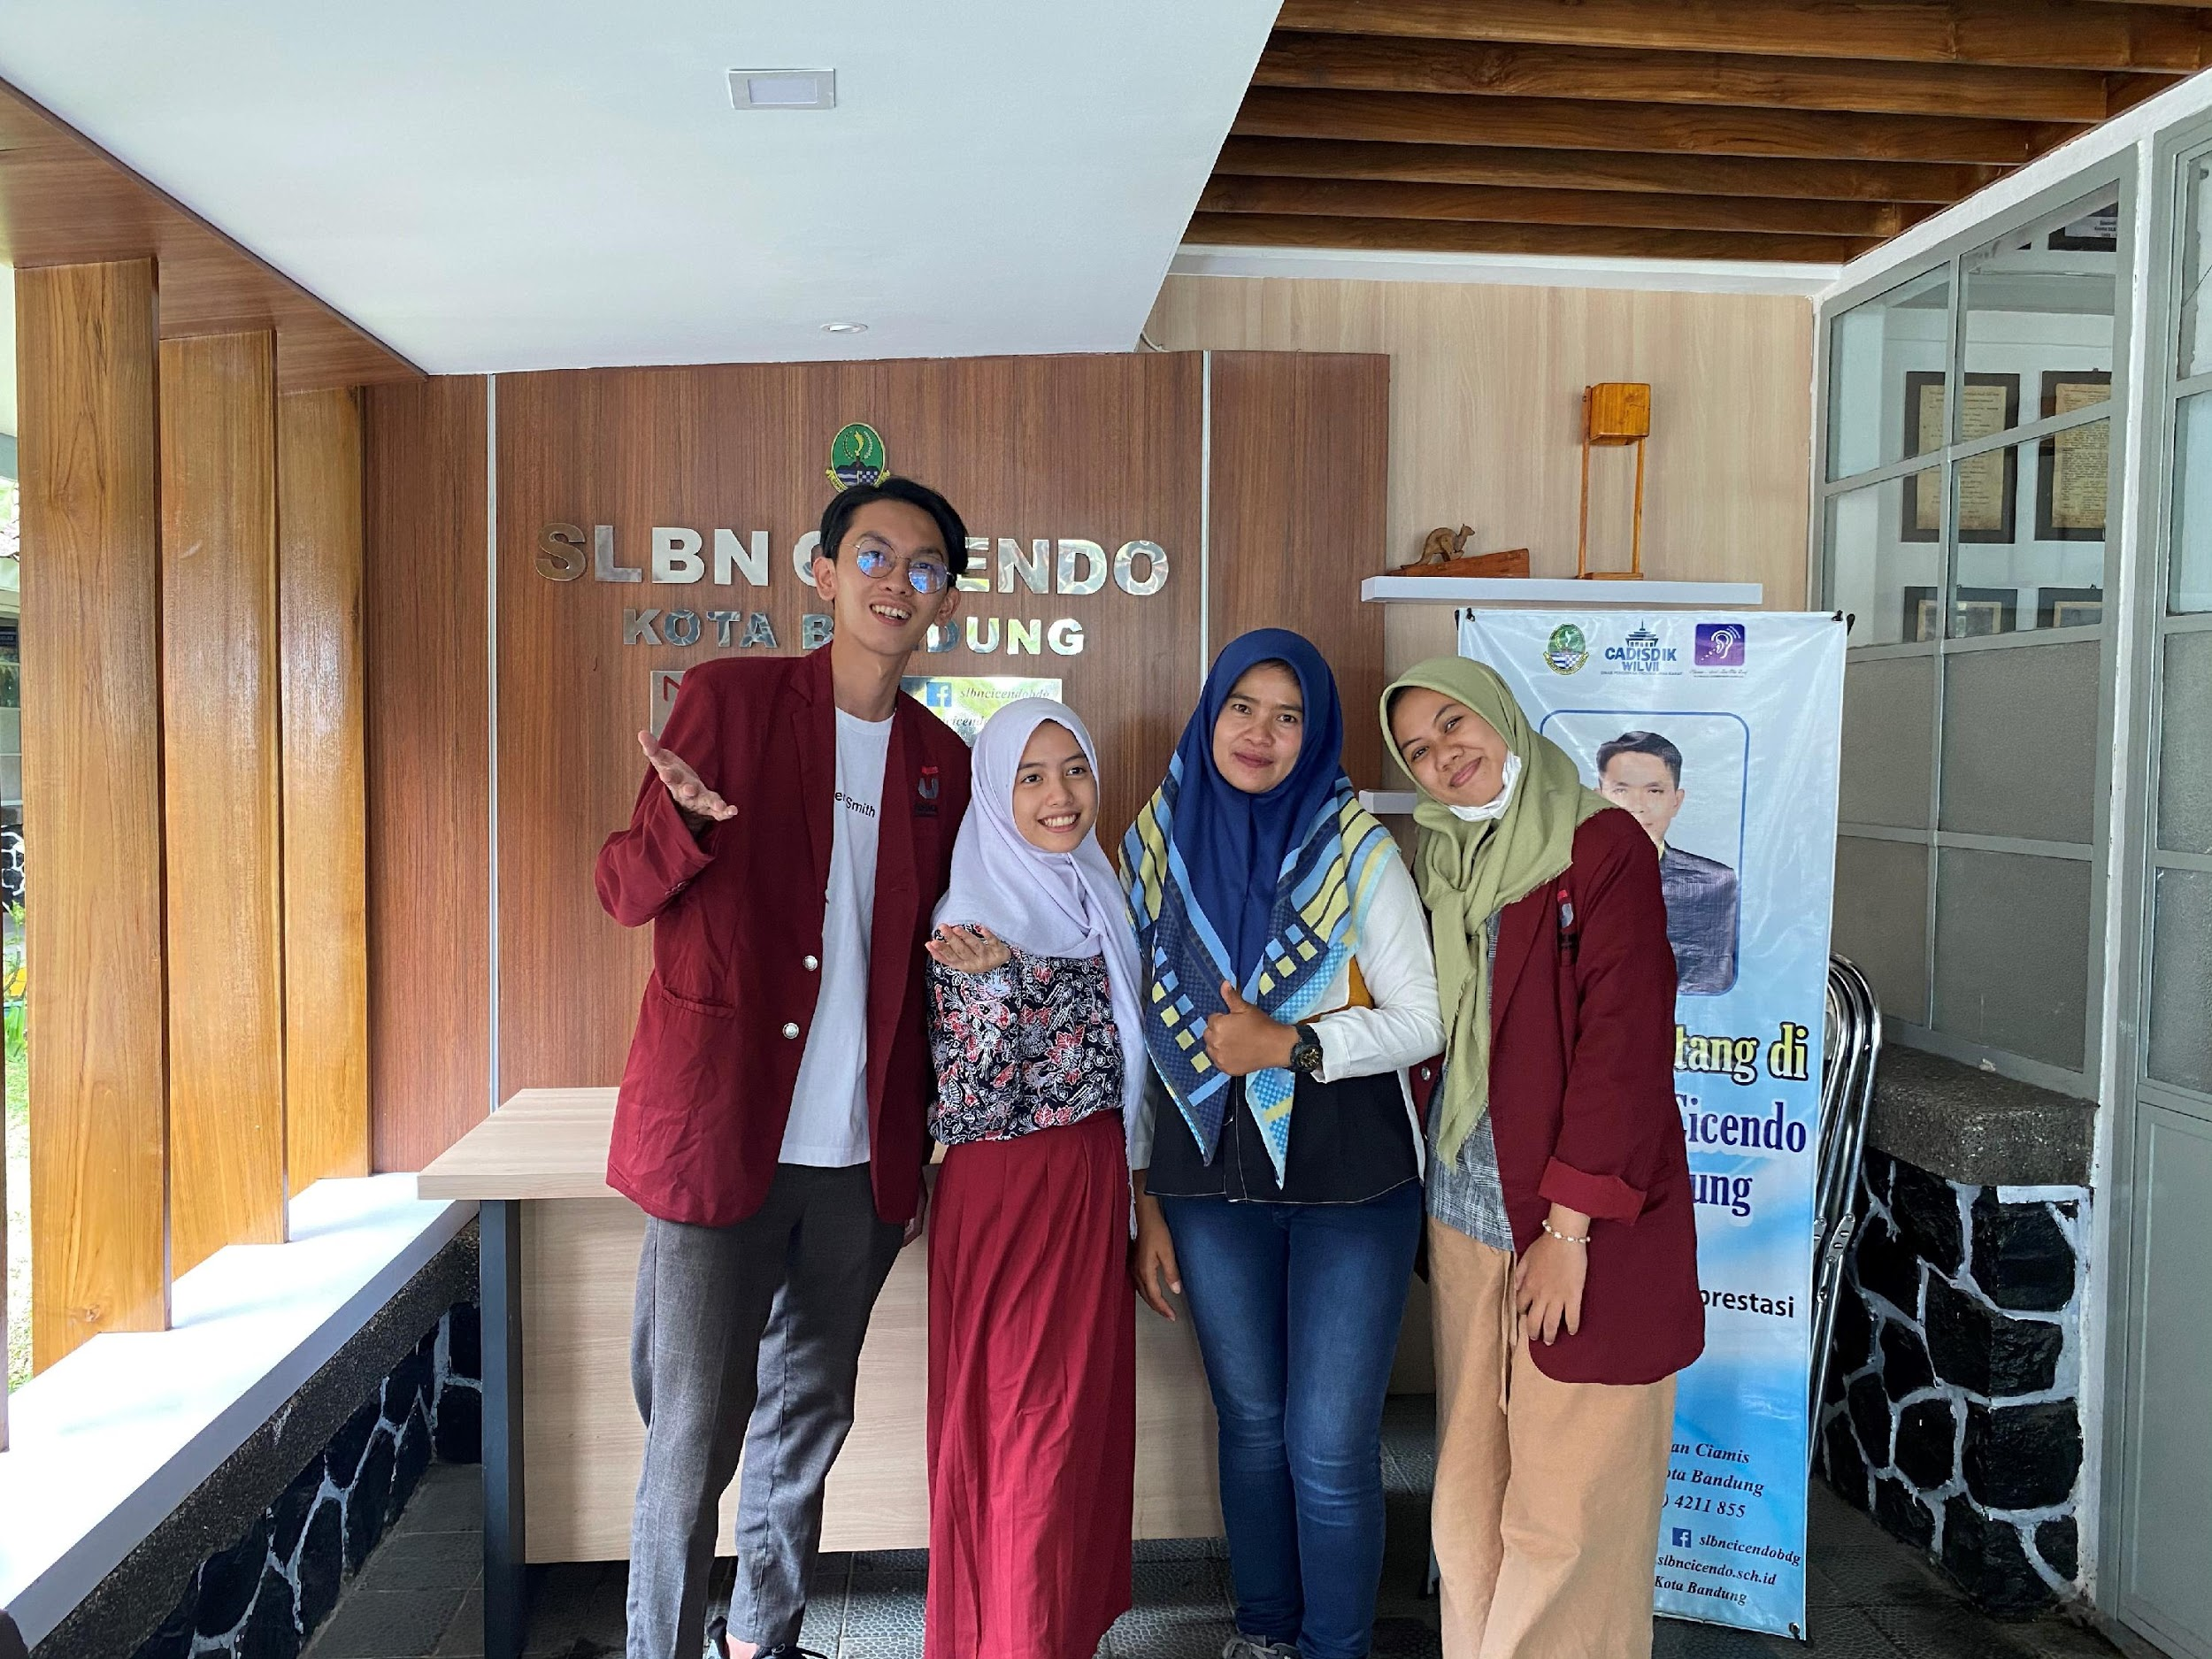
\includegraphics[width=0.8\textwidth]{lampiran-a-2}
    \caption{Foto bersama siswa yang diwawancarai dan orang tuanya.}
    \label{fig:lampiran-a-2}
\end{figure}

\begin{figure}[H]
    \centering
    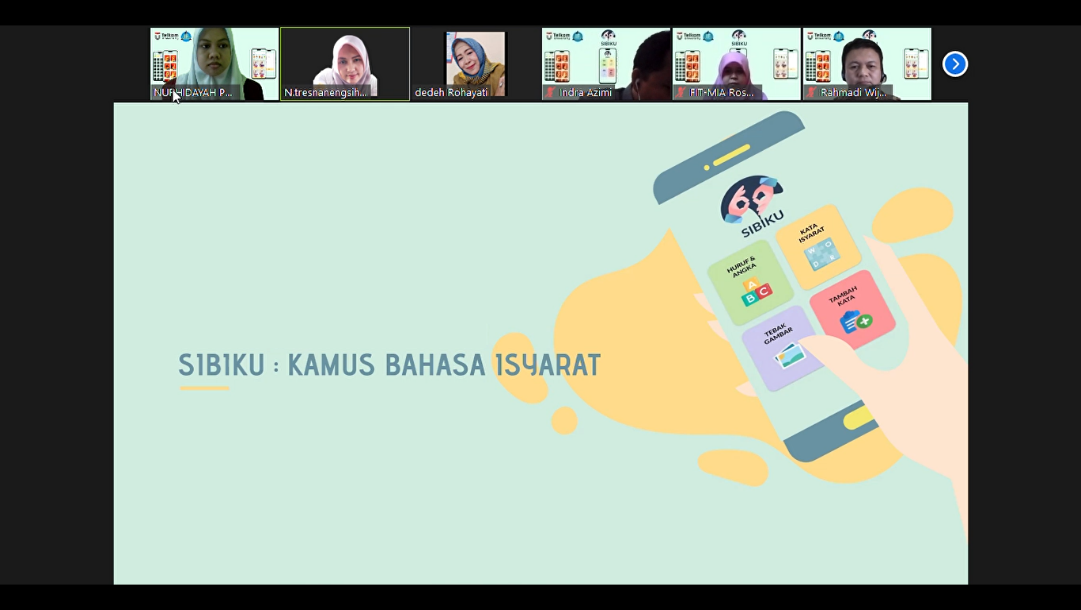
\includegraphics[width=0.8\textwidth]{lampiran-a-3}
    \caption{Sosialisasi aplikasi SIBIKU ke pengguna melalui Zoom.}
    \label{fig:lampiran-a-3}
\end{figure}

\begin{figure}[H]
    \centering
    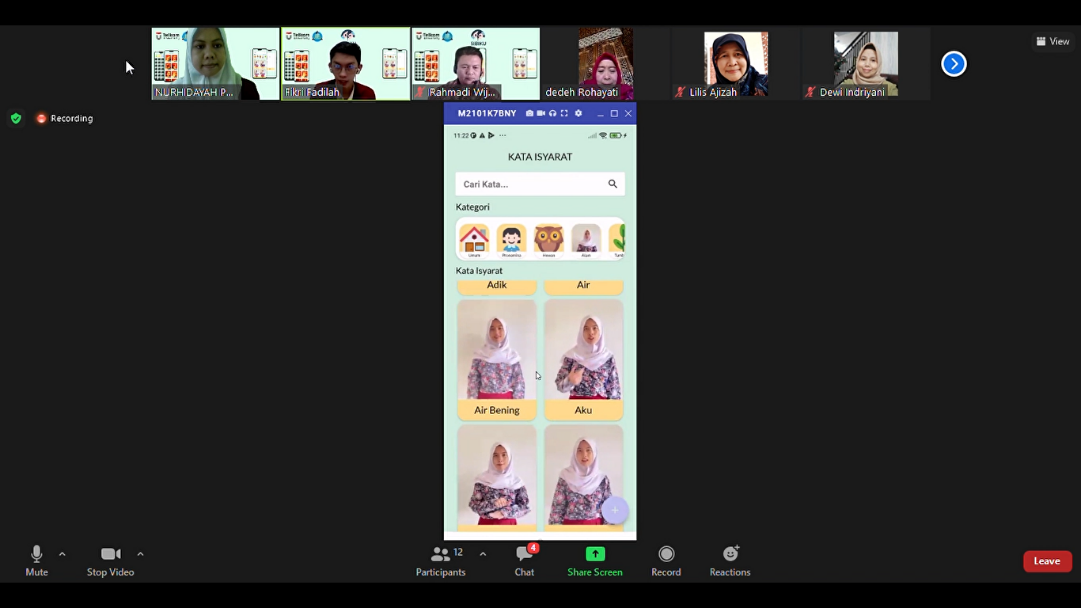
\includegraphics[width=0.8\textwidth]{lampiran-a-4}
    \caption{Pengguna mencoba aplikasi di smartphone masing-masing dan mengisi kuesioner.}
    \label{fig:lampiran-a-4}
\end{figure}

\chapter{Perhitungan Usability Test}
\label{sec:lampiran-perhitungan}
Berikut adalah perhitungan hasil usability test dengan skala Likert
(STS=1, TS=2, N=3, S=4, SS=5).

\begin{longtable}{|c|p{5.5cm}|c|c|c|c|c|c|c|c|c|c|c|}
    \caption{Perhitungan Usability Test} \\
    \hline
    \textbf{No} & \textbf{Pertanyaan} & \multicolumn{5}{c|}{\textbf{Skor Likert}} & \multicolumn{5}{c|}{\textbf{Total Skor Likert}} & \textbf{\%} \\ \cline{3-12}
     & & STS & TS & N & S & SS & STS & TS & N & S & SS & \\ \hline
    \endfirsthead
    \hline
    \textbf{No} & \textbf{Pertanyaan} & \multicolumn{5}{c|}{\textbf{Skor Likert}} & \multicolumn{5}{c|}{\textbf{Total Skor Likert}} & \textbf{\%} \\ \cline{3-12}
     & & STS & TS & N & S & SS & STS & TS & N & S & SS & \\ \hline
    \endhead
    \multicolumn{13}{|c|}{\textbf{Effectiveness}} \\ \hline
    1 & Apakah setuju Kamus SIBI sangat cukup dan efektif digunakan dalam kegiatan belajar pada siswa/i SLB? & 0 & 1 & 8 & 22 & 40 & 0 & 2 & 24 & 88 & 200 & 88,5 \\ \hline
    2 & Apakah setuju jika Kamus SIBI dibuat dalam bentuk aplikasi? & 0 & 1 & 7 & 13 & 50 & 0 & 2 & 21 & 52 & 250 & 91,5 \\ \hline
    3 & Apakah setuju aplikasi Kamus SIBI sangat diperlukan saat ini? & 0 & 0 & 8 & 19 & 44 & 0 & 0 & 24 & 76 & 220 & 90,1 \\ \hline
    4 & Apakah setuju dengan adanya aplikasi Kamus SIBI dapat meningkatkan semangat belajar? & 0 & 0 & 7 & 22 & 42 & 0 & 0 & 21 & 88 & 210 & 89,9 \\ \hline
    5 & Apakah setuju aplikasi Kamus SIBI dapat membantu permasalahan yang ada pada SLB? & 0 & 0 & 10 & 21 & 40 & 0 & 0 & 30 & 84 & 200 & 88,5 \\ \hline
    \multicolumn{12}{|r|}{\textbf{Rata-Rata}} & \textbf{89,7} \\ \hline
    \multicolumn{13}{|c|}{\textbf{Usefulness}} \\ \hline
    1 & Setelah menggunakan aplikasi SIBIKU, aplikasi sangat mudah untuk digunakan & 0 & 0 & 8 & 21 & 42 & 0 & 0 & 24 & 84 & 210 & 89,6 \\ \hline
    2 & Aplikasi SIBIKU dapat membantu dalam pembelajaran kosakata bahasa isyarat & 0 & 0 & 7 & 16 & 48 & 0 & 0 & 21 & 64 & 240 & 91,5 \\ \hline
    3 & Aplikasi SIBIKU mempermudah proses belajar mengajar bahasa isyarat saat ini & 0 & 0 & 6 & 21 & 44 & 0 & 0 & 18 & 84 & 220 & 90,7 \\ \hline
    4 & Fitur yang ada pada aplikasi SIBIKU sangat membantu menyelesaikan permasalahan yang ada & 0 & 0 & 8 & 29 & 34 & 0 & 0 & 24 & 116 & 170 & 87,3 \\ \hline
    5 & Aplikasi terorganisir dengan baik & 0 & 0 & 11 & 22 & 38 & 0 & 0 & 33 & 88 & 190 & 87,6 \\ \hline
    \multicolumn{12}{|r|}{\textbf{Rata-Rata}} & \textbf{89,4} \\ \hline
    \multicolumn{13}{|c|}{\textbf{Satisfaction}} \\ \hline
    1 & Tampilan pada aplikasi SIBIKU sangat bagus dan menarik & 0 & 1 & 7 & 21 & 42 & 0 & 2 & 21 & 84 & 210 & 89,3 \\ \hline
    2 & Desain antar muka bagus dan mudah dipahami & 0 & 0 & 9 & 19 & 43 & 0 & 0 & 27 & 76 & 215 & 89,6 \\ \hline
    3 & Penggunaan warna pada aplikasi bagus dan menarik & 0 & 1 & 6 & 23 & 41 & 0 & 2 & 18 & 92 & 205 & 89,3 \\ \hline
    4 & Icon pada aplikasi sesuai dan mudah dipahami & 0 & 1 & 5 & 21 & 44 & 0 & 2 & 15 & 84 & 220 & 90,4 \\ \hline
    5 & Desain sesuai dengan anak-anak & 0 & 1 & 7 & 15 & 48 & 0 & 2 & 21 & 60 & 240 & 91,0 \\ \hline
    \multicolumn{12}{|r|}{\textbf{Rata-Rata}} & \textbf{89,9} \\ \hline
\end{longtable}

\end{document}
